\documentclass[preprint,12pt]{article}
\usepackage[utf8]{inputenc}




\usepackage{titling}

\usepackage{nomencl}
%Math setting
\usepackage{bm} %bold math 
\usepackage{amsmath}% typesetting math
%\usepackage{siunitx}% typesetting units
\usepackage{esint} % various fancy integral symbols
%Cite setting
\usepackage{cleveref} %for several ref at text
\usepackage{xfrac}
%multi figure

\usepackage[section]{placeins} % to ensure picture is in the same section
\usepackage{lscape}%to use lanskape page

\usepackage{multirow} % Table multirow
\setcounter{secnumdepth}{5} %depth toc
\setcounter{tocdepth}{5}

\usepackage{xcolor} %change font color
%reference
\usepackage{natbib}
% If want to use bib at each chapter
%\usepackage[sectionbib]{chapterbib}
%\usepackage{chapterbib}
%\usepackage[nottoc]{tocbibind}  % to make it appear at table of content

\usepackage{graphicx}
\usepackage{booktabs}
\usepackage[T1]{fontenc}
\usepackage{mathptmx}
\usepackage{float}
\usepackage{amssymb}
\usepackage{graphicx}
\usepackage{listings}
\usepackage{graphics}
\usepackage[outdir=./]{epstopdf}
\usepackage{stackengine}
\newcommand\xrowht[2][0]{\addstackgap[.5\dimexpr#2\relax]{\vphantom{#1}}}

\usepackage{pdfpages}
\usepackage{mathtools}
\DeclarePairedDelimiter\abs{\lvert}{\rvert}%
\usepackage{cancel}


\usepackage{lscape}
\usepackage{multirow}
\usepackage{subfigure}
\usepackage{amsmath}
\usepackage{amsfonts}

\usepackage{adjustbox}
\usepackage{tikz}
\usetikzlibrary{shapes.geometric, arrows}
\usetikzlibrary{calc}


\tikzstyle{startstop} = [rectangle, rounded corners, minimum width=3cm, minimum height=1cm,text centered, draw=black, fill=red!30]

\tikzstyle{io} = [trapezium, trapezium left angle=70, trapezium right angle=110, minimum width=3cm, minimum height=1cm, text centered,text width=4cm, draw=black, fill=blue!30]

\tikzstyle{process} = [rectangle, minimum width=3cm, minimum height=1cm, text centered, text width=7cm, draw=black, fill=orange!30]

\tikzstyle{process0} = [rectangle, minimum width=3cm, minimum height=1cm, text centered, text width=3cm, draw=black, fill=orange!30]

\tikzstyle{decision} = [diamond, minimum width=3cm, minimum height=1cm, text centered,text width=2.5cm, text height=0.1cm, draw=black, fill=green!30]
\tikzstyle{connect} = [circle, minimum width=0.1cm, minimum height=0.1cm, text centered, draw=black, fill=green!30]

\tikzstyle{arrow} = [thick,->,>=stealth]

% \captionsetup{compatibility=false}

\newcommand\tab[1][1cm]{\hspace*{#1}}
\newcommand\xrowht[2][0]{\addstackgap[.5\dimexpr#2\relax]{\vphantom{#1}}}
\usepackage{caption}
\usepackage{subcaption}
\usepackage[medium]{titlesec}
\title{Complex wave structure interaction using Hybrid coupling potential and viscous solvers}
\date{\vspace{-5ex}}

\begin{document}


% Please add the following required packages to your document preamble:
% \usepackage{graphicx}
% Please add the following required packages to your document preamble:
% \usepackage{graphicx}

%%%%%%%%%%%%%%%%%%%%%%%%%%%%%%%%%%%%%%%%%%%%%%%%%%%%%%%%%%%%%%%%%%%%%%%%%%%%%%%%
%% Commenting IIT Madras introduction page%%%%%%%%%%%%%%%%%%%%%%%%%%%%%%%%%%%%

\begin{table}[]
\centering
\resizebox{\textwidth}{!}{%
\begin{tabular}{lll}
\multicolumn{2}{c}{\textbf{RESEARCH PROPOSAL MEETING REPORT}}           &  \\\xrowht{15pt}
\multicolumn{2}{c}{\textbf{Data Sheet}}                                 &  \\\xrowht{15pt}
\textbf{Name}                  & : SITHIK A                             &  \\\xrowht{15pt}
\textbf{Registration No}       & : OE17D027                             &  \\\xrowht{15pt}
\textbf{Department}            & : Ocean Engineering                    &  \\\xrowht{15pt}
\textbf{Date of Joining}       & : 02-01-2018                           &  \\\xrowht{15pt}
\textbf{Specialization/Stream}             & : Hydrodynamics of complex wave structure      &                                    \\\xrowht{15pt}
\textbf{Area of Research work}             & : Coupling Potential and viscous flow theories &                                    \\\xrowht{15pt}
\textbf{Category of Admission} & : HTRA                                 &  \\\xrowht{15pt}
\textbf{Guide}                 & : Dr. V.Sriram and Prof.Pierre Ferrant &  \\\xrowht{15pt}
\multicolumn{1}{l}{\textbf{Date of DC meetings:}}                       &  \\ \hline
\multicolumn{1}{|c|}{\textbf{Description}} & \multicolumn{1}{c|}{\textbf{Event}}            & \multicolumn{1}{c|}{\textbf{Date}} \\ \hline
\multicolumn{1}{|c|}{1st DC meeting}       & \multicolumn{1}{c|}{Comprehensive Viva}        & \multicolumn{1}{c|}{08-04-2019}    \\ \hline
                               &                                        & 
\end{tabular}%
}
\end{table}
% Please add the following required packages to your document preamble:
% \usepackage{graphicx}
\textbf{Details of Course Work: }
\begin{figure}[H]
    \centering
    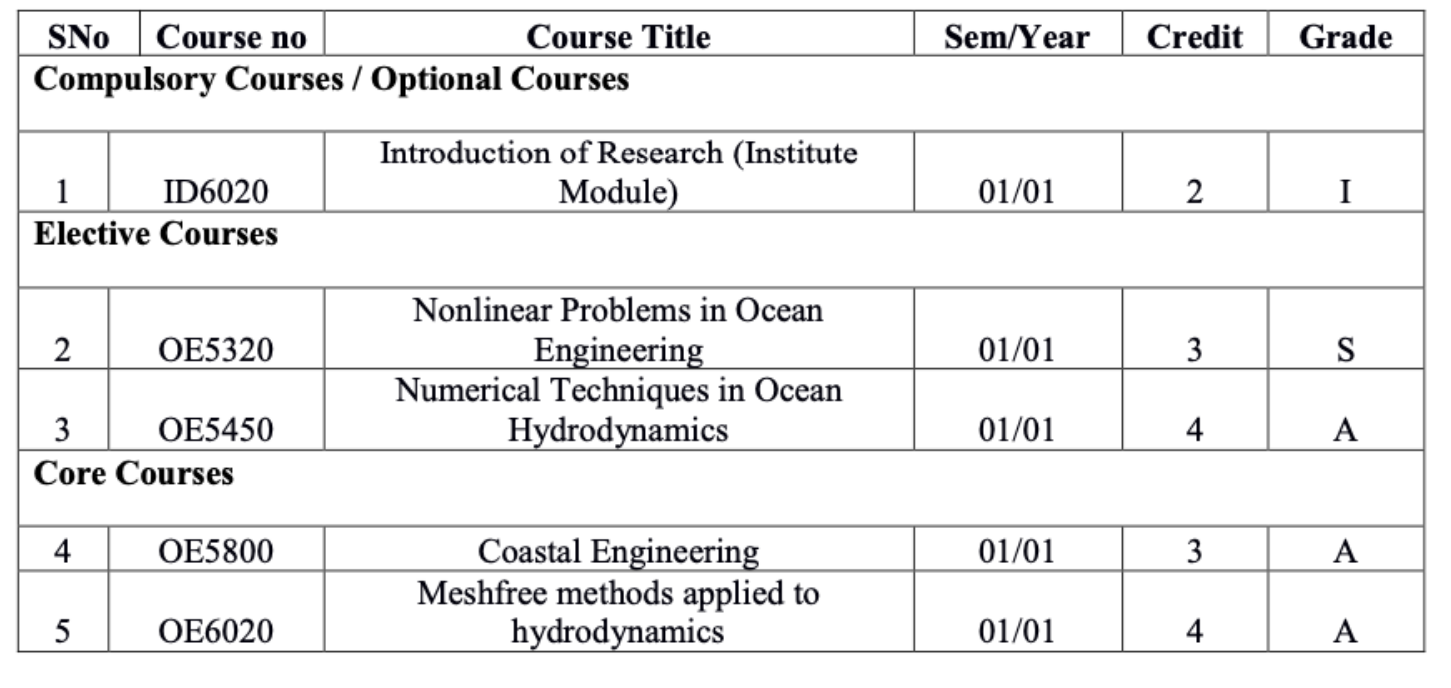
\includegraphics[width=\textwidth]{RPS.png}
    \label{fig:my_label}
\end{figure}

\textbf{Signature of Scholar} \tab \tab \tab \tab \tab \textbf{Signature of Guide}

{\fontfamily{ptm}\selectfont


\section{Introduction}
 Installation of any offshore structures for harvesting energy or for oil and gas industries is still burdensome because of rough sea state. Unless there is calm water condition prevailing it is very difficult to install any substructure or floating structure at offshore sites. Hence, there has been a great potential for research to investigate the installation of offshore structures for normal and for more energetic wave conditions. To understand and develop the methodology for the installation, the hydrodynamic response of the structure and impact received by the offshore crane is vital. In this context the research study will be  focused on the installation of offshore wind energy sub structures under wave conditions.
\par
This type of  wave -structure interaction problem can be assessed by various approaches. Empirical formulations, model tests in wave tanks and numerical simulation methods are all frequently used. The numerical simulation approach for the wave-structure interaction problem refers to the use of computer software and numerical analysis methods to solve and analyze the fluid flow and its interaction with the structure. The numerical simulation methods have been developed since they are able to assess complex problems where no empirical formulations exist, and their cost is often much less than a wave tank test. \par
Commercial software packages such as WAMIT, ANSYS,STAR-CCM+, Open foam etc. are available for wave structure interaction type of problems. The methods for the fluid simulation behind these software packages can be distinguished into two general groups by whether the viscosity of the fluid is considered or not. Potential theory is widely used if the fluid is assumed to be inviscid. Otherwise, the viscous flow is modelled by Navier-Stokes (NS) equations and solved with Computational Fluid Dynamics (CFD) approaches . 
The potential flow solvers(Boundary Element Method(BEM), Finite Element Method(FEM), Finite Difference Method(FDM), Mesh-free methods etc) are efficient and accurate when the geometry of the structure is smooth and the viscous effects are negligible. However, the irrotational flow assumption of potential theory can lead to numerical difficulties in realistic wave-structure interaction scenario when the flow separation happens. \par
For this reason, numerous viscous flow solvers with the Computational Fluid Dynamics (CFD) approach are developed to assess the wave-structure interaction problem by solving NS equations.Numerous validations have proved that viscous CFD solvers are able to provide high fidelity results for a wide variety of applications . Practical marine and ocean engineering applications need sufficiently long simulation time resulting in a prohibitive computational cost (very high than potential solvers). \par
 
The objective of the research is to develop an accurate and efficient numerical method to simulate the complex wave structure interaction problem by coupling the viscous and potential flow models. Hence two solvers are chosen foamStar and SWENSE - each based on the different philosophies that will be  explained later. Both the solvers will be improved and modified to capable of doing complex wave structure interaction problems. Validation of solvers will be done with the experiments carried out in the wave basin. 



\section{Literature Review}
For highly accurate study of wave transformation, wave-breaking and fluid-structure interaction processes, the computational cost is tremendously high when using a single 3D CFD model and its application is unfeasible for large domain \cite{Vandebeek2018}. Thus, in recent years, a considerable research effort has been made on developing near-far field coupled models that were able to deal with the above issue in an efficient way.  Coupled models have been generally classified based on the physics involved. Four categories can be identified with respect to the  governing equations being solved such as,  FNPF(Fully Nonlinear Potential Flow models), CFD(NS based Computational Fluid Dynamics model), NLSW(NonLinear Shallow Water equations models) and BT(Boussinesq -type models). The short summary of researches carried out in these coupled models with its coupling type are mentioned in Table \ref{General_models}.Although the use of BT or non-hydrostatic NLSW codes for wave transformation has been common practise, the application of CFD allows to reduce uncertainties in hydrodynamic modelling as the full set of NS equations is being solved.  In general, several FNPF-CFD coupled models have been developed by the scientific community over the years because of its robustness. There are two ways this coupling can be carried out, one is domain decomposition and other is functional decomposition. Each methods will be discussed in detail in the following sections. The summary of the  previous research carried over the years in FNPF-CFD coupling models are detailed in Table \ref{DDandFD}. 



% Please add the following required packages to your document preamble:
% \usepackage{graphicx}
\begin{table}[]
\centering
\resizebox{1.1\textwidth}{!}{%
\begin{tabular}{llllll}
\multicolumn{1}{c}{}      & \multicolumn{1}{c}{} &               & \multicolumn{1}{c}{} & \multicolumn{1}{c}{} & \multicolumn{1}{c}{} \\ \hline
\multicolumn{1}{c}{\textbf{Authors}} &
  \multicolumn{1}{c}{\textbf{Models}} &
  \textbf{\begin{tabular}[c]{@{}l@{}}Transfer \\ type\end{tabular}} &
  \multicolumn{1}{c}{\textbf{\begin{tabular}[c]{@{}c@{}}Coupling \\ way\end{tabular}}} &
  \multicolumn{2}{c}{\textbf{Numerical model}} \\ \cline{5-6} 
\multicolumn{1}{c}{} &
  \multicolumn{1}{c}{} &
   &
  \multicolumn{1}{c}{} &
  \multicolumn{1}{c}{\textbf{Model 1}} &
  \multicolumn{1}{c}{\textbf{Model 2}} \\ \hline
Separate Table (Table \ref{DDandFD})    & FNPF-CFD             & BC \& Overlap & One/Two way          & FNPF                 & CFD                  \\
Mintgen and Manhart et al\cite{Mintgen2018} & SWE-CFD              & BC            & Two way              & FVM                  & FVM                  \\
Altomare et al\cite{Altomare2014}            & NLSW-CFD             & BC            & One way              & FDM                  & SPH                  \\
Kassiotis et al\cite{Kassiotis2011}           & BT - CFD             & BC \& Overlap & Oneway               & FDM                  & SPH                  \\
Kumar et al\cite{Kumar2015}               & CFD-CFD(3D)          & Overlap       & One way              & SPH                  & FVM                  \\
El Safti et al \cite{ElSafti2014}            & CFD-CFD(2D-3D)       & Overlap       & One way              & FVM                  & FVM                  \\
Ferrar et al \cite{MartinezFerrer2016}             & CFD-CFD(3D-3D)       & BC            & Two way              & FVM                  & FVM                  \\
Di Paolo et al \cite{DiPaolo2020}\cite{DiPaolo2020a}           & CFD-CFD(2D-3D)       & BC            & One/Two way          & FVM                  & FVM                  \\ \hline
\end{tabular}%
}
\caption{Tabulated Overview of existing coupled models. FNPF- Fully Nonlinear Potential Flow models, CFD - NS based Computational Fluid Dynamics, SWE- Shallow Water Equations, NLSW-NonLinear Shallow Water equations, BT- Boussinesq -type ,BCs stands for boundary conditions, while overlap refers to the use of overlapping zones at the interfaces between the different models}
\label{General_models}
\end{table}

\begin{table}[]
\begin{tabular}{ccccc}
                                                                                      &                        &                                                                  &                       &                      \\ \hline
\textbf{Previous research}                                                            & \textbf{Decomposition} & \textbf{\begin{tabular}[c]{@{}c@{}}Coupling \\ way\end{tabular}} & \multicolumn{2}{c}{\textbf{Numerical model}} \\ \cline{4-5} 
                                                                                      &                        &                                                                  & \textbf{phi}          & \textbf{NS}          \\ \hline
Guignard et al\cite{Guignard1999}                                                                        & Domain                 & One                                                              & BEM                   & FVM                  \\
\begin{tabular}[c]{@{}c@{}}Lachaume et al (2003)\cite{Lachaume2003}, \\ Grilli et al (2004) \cite{Grilli2004}\end{tabular} & Domain                 & One                                                              & BEM                   & FVM                  \\
Christensen et al (2009) \cite{Christensen2009}                                                              & Domain                 & One                                                              & phiI                  & FVM                  \\
Jacobsen et al (2012)\cite{Jacobsen2012}                                                                 & Domain                 & One                                                              & phiI                  & FVM                  \\
Hilderbrandt et al (2013) \cite{Hildebrandt2013}                                                             & Domain                 & One                                                              & FEM                   & FVM                  \\
Higuera et al (2013) \cite{Higuera2013}                                                                  & Domain                 & One                                                              & phiI                  & FVM                  \\
Paulsen et al (2014) \cite{Paulsen2014}                                                                  & Domain                 & One                                                              & FDM                   & FVM                  \\
Duz et al (2016) \cite{Duz2016}                                                                      & Domain                 & One                                                              & FDM                   & FVM                  \\
\begin{tabular}[c]{@{}c@{}}foamStar\\ Monroy et al (2016) \cite{Monroy2016} \end{tabular}                & Domain                 & One                                                              & phiI, HOS             & FVM                  \\ \hline
Tahara et al (1992)\cite{TAHARA199233}                                                                    & Domain                 & Two                                                              & BEM                   & FVM                  \\
Campana et al (1992) \cite{campana1992}                                                                  & Domain                 & Two                                                              & BEM                   & FVM                  \\
Campana et al (1995) \cite{Campana1995}                                                                  & Domain                 & Two                                                              & BEM                   & FVM                  \\
Chen and Lee (1999) \cite{Chen1999}                                                                  & Domain                 & Two                                                              & BEM                   & FVM                  \\
Guillerm (2001) \cite{Guillerm2001}                                                                     & Domain                 & \textit{Two}                                                     & Poincare              & \textit{FDM}         \\
Iafrati and Campana(2003) \cite{Iafrati2003}                                                             & Domain                 & Two                                                              & BEM                   & FVM                  \\
Colicchio et al (2006) \cite{Colicchio2006}                                                                & Domain                 & Two                                                              & BEM                   & FVM                  \\
Hamilton and Yeung (2011) \cite{Hamilton2011}                                                             & Domain                 & Two                                                              & Shell func            & FVM                  \\
Sriram et al(2014) \cite{Sriram2014}                                                                   & Domain                 & Two                                                              & FEM                   & IMLPG                \\
Fredriksen (2015)\cite{Fredriksen2015}                                                                    & Domain                 & Two                                                              & HPC                   & FVM                  \\
Lu et al (2016) \cite{Lu2016}                                                                      & Domain                 & Two                                                              & FVM                   & FVM                  \\
Siddique et al (2017)\cite{Siddiqui2017}                                                                 & Domain                 & Two                                                              & HPC                   & FVM                  \\
Verbrugghe et al (2018) \cite{Verbrugghe2018}                                                               & Domain                 & Two                                                              & FDM                   & SPH                  \\ \hline
Kim et al (2005) \cite{Kim2005}                                                                     & Functional I           & One                                                              & BEM                   & FVM                  \\
Kim et al (2011) \cite{Kim2005a}                                                                     & Functional I           & One                                                              & phiI                  & FVM                  \\
Edmund (2012) \cite{Edmund2013}                                                                         & Functional I           & Two                                                              & BEM                   & FVM                  \\
Rosemurgy (2014)\cite{Rosemurgy2016}                                                                      & Functional I           & Two                                                              & BEM                   & FVM                  \\ \hline
Ferrant et al (2003) \cite{Ferrant2002}                                                                 & Functional II          & One                                                              & phiI                  & FDM                  \\
Gentaz et al (2004) \cite{Gentaz2004}                                                                   & Functional II          & One                                                              & phI                   & FVM                  \\
Luquet et al(2007) \cite{Luquet2007}                                                                   & Functional II          & One                                                              & phiI                  & FVM                  \\
Vukcevic (2016)\cite{Vukcevic2016}                                                                       & Functional II          & One                                                              & phiI                  & FVM                  \\
Li (2020) \cite{zhaobin_progress}                                                                             & Functional II          & One                                                              & HOS                   & FVM                  \\ \hline
\end{tabular}
\caption{Summary of previous research on the coupling of potential/viscous flows; BEM(Boundary Element Method), FVM(Finite Volume Method), FDM(Finite Difference Method), HOS(Higher Order Spectral method)}
\label{DDandFD}
\end{table}


\begin{figure}[]
 \centering 
 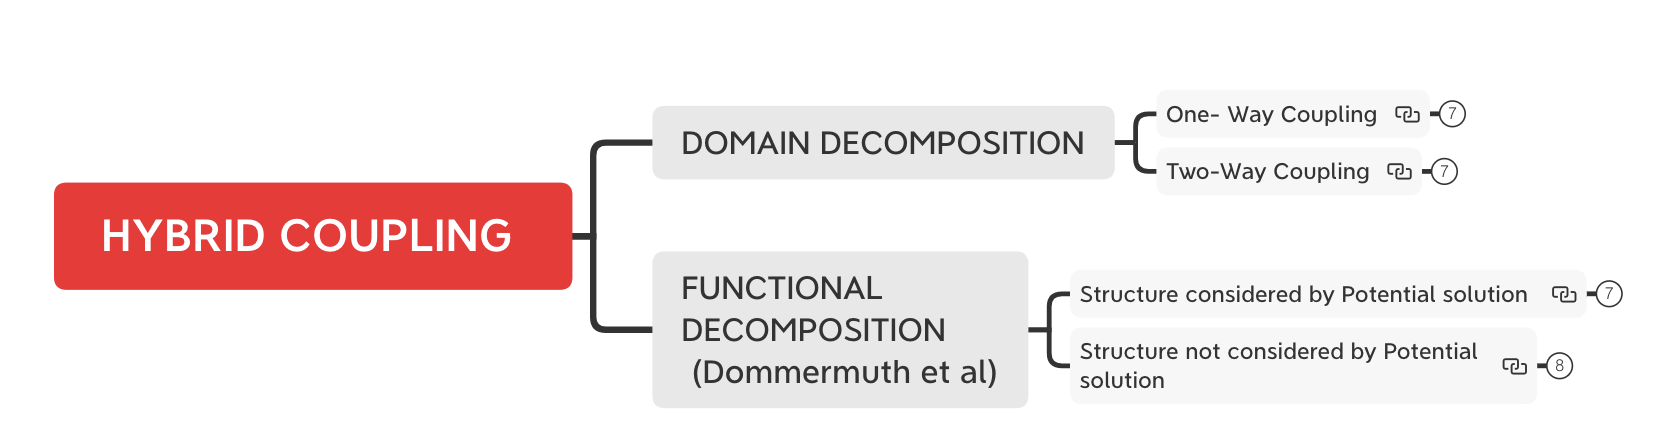
\includegraphics[width=\textwidth]{HYBRID_COUPLING1.png}
 \caption{General Classification of FNPF-CFD coupling}
\end{figure}


\subsection{Domain decomposition (DD)}
\begin{figure}
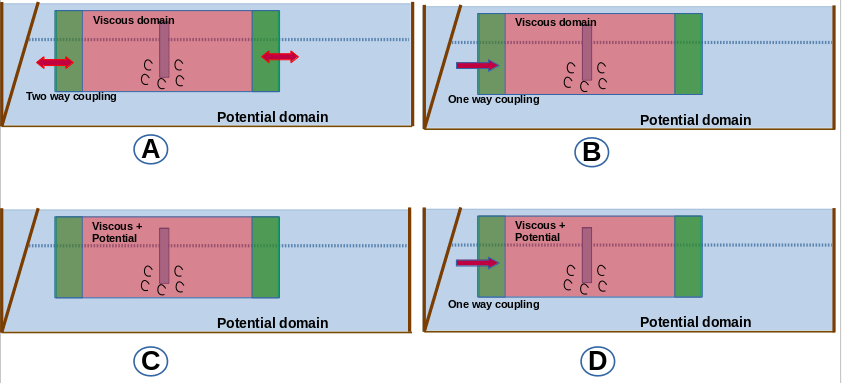
\includegraphics[width=\textwidth]{SWENSE.jpg}
\caption{Potential and viscous flow coupling methods with description. A: Domain decomposition with two way coupling; B: Domain decomposition with one way coupling; C: Functional decomposition of viscous domain; D: SWENSE - One way domain decomposition and functional decomposition of viscous domain}
\label{coupling}
\end{figure}

In domain decomposition, as shown in the Figure \ref{coupling}, computational domain is split into parts and in each part appropriate solver is used for solving the governing equation. In the wave-structure interaction problem, viscous effects and wave nonlinearities are strong in the vicinity of body surface. Even though the generated vortex propagates up to relatively far-field, it is possible to decompose the computational domain into viscous inner sub-domain and potential outer sub-domain. Both two-way and one-way coupling methodologies are applicable with different coupling regions. In the coupling region, the information is delivered from viscous/potential flow to the other. It is usually categorized into direct and overlapped coupling regions. The direct coupling region represents that two flows share one surface to deliver each of the flow quantities to the other\cite{Paulsen2014}. The overlapped coupling regions refers to that the information transfer happens at two distinct boundary surfaces with distance or the volumic blending zones. In the volumic blending zone, the weight function is applied for smooth transition of flow quantities. Therefore, information delivery is done in different places \cite{Vandebeek2018}. Pressure, fluid velocity and surface elevation are most general values to be exchanged between the solvers. \par
Based on how the information between the solvers is being transferred, it can be either one way coupling (weakly coupling) and two way coupling (strong coupling). In one way coupling information/values are transferred in one way from the potential solver into the viscous solver, but in two way coupling, the information/values transferred in both ways (from potential to viscous and also from viscous to potential solvers). The two-way coupling is beneficial since the size of the computational domain of the viscous solver can be drastically reduced. But it requires iterations between the two sub-domains on the common interface. But the advantage of one way coupling is no such iterations are needed.Therefore, one-way coupling is commonly used nowadays by imposing the incident waves as the boundary condition \cite{Jacobsen2012},\cite{Paulsen2014}. Although one way coupling need larger viscous domain to avoid the influence of boundaries. Two phase CFD solver \textit{foamStar} is one of the example for one way domain decomposition developed by Ecole Centrale Nantes as inhouse code, used in this research work. Its theory and functioning is described in the next section. 
 

\subsection{Functional decomposition (FD)}
In this approach, the total problem is split into potential component and a viscous component that co-exist in the same computation domain as shown in Figure \ref{coupling}. These individual components are solved with different governing equation and different solvers, say BEM/HOS for potential solvers and FVM for viscous solvers. There are two categories of coupling in this decomposition based on the fact whether structure is considered in the potential flow solution or not. In the Functional I category as mentioned in the Table \ref{DDandFD}, it involves solving entire problem by potential solver and viscous contribution is added as correction from the viscous solver. The advantage in this method is viscous solver needs to focus only on viscous effects near the structure and in the wake. But still same numerical difficulties will be encountered by the potential solver when the structure and flow is complex . \par
In the Functional II category, total solution is divided into Incident solution and complementary solution : the incident solution is derived from potential part of the solution, and complementary solution is derived from viscous solver by solving complementary part equation. This approach been proposed as Spectral Wave Explicit Navier Stokes Equations(SWENSE) in the work of Luquet et al \cite{Luquet2007}. This method has been improved in years from Single phase viscous solver in coupling with stream function theory (Ferrant et al \cite{Ferrant2002}, Luquet et al \cite{Luquet2003}, Gentaz et al \cite{Gentaz2004}, Monroy et al\cite{Monroy2010}) to Multi-phase solver and also coupling with domain decomposition strategy (Luquet et al \cite{Luquet2007}, Vukcevic et al \cite{Vukcevic2016}). The work has been reformulated SWENSE in multi-phase flow by decomposing a level-set and fluid velocity, later Li et al \cite{zhaobin_progress} applied a similar approach with extended incident pressure for VOF field. \par

The advantage of using the incident wave solution as the potential solution part is its simplicity and robustness: no more numerical difficulties are expected in the potential part since it is given directly by wave models.Since scattered waves far from the structure is not of interest, \textbf{coarse mesh can be used in the far-field to reduce the computational cost}. The original single-phase SWENSE method reduced the CPU time by a factor of 50 compared with direct CFD method for an equivalent precision \cite{Gentaz2004}.  In this research work, application and development of SWENSE (Functional II) coupled with potential solver in one way domain decomposition will be carried out.



\section{Research Gap}
The success of the SWENSE method to speed up single-phase CFD solvers encourages researchers to extend the method for two-phase solvers to enhance their performance on wave related problems.The coupling of a single-phase potential solver and a two-phase viscous solver exists in the literature, but mostly remains in the domain decomposition category. This difficulty had limited the development of two-phase SWENSE method for a longtime. The first attempt to develop a two-phase SWENSE method was made by Vukčević et al \cite{Vukcevic2016}. However, their method is different from the original SWENSE method and still requires refined mesh to keep the incident wave accurate. Zhaobin et al \cite{zhaobin_progress} developed a two phase model as explained in the previous section with keeping the advantage of using coarse mesh for the wave propagation to enhance the viscous solvers performance, but still the  formulation is to be validated for the breaking waves and steep waves. Also the coupling for SWENSE is carried out is only for Higher Order Spectral Method(\cite{DUCROZET201219})as potential solver  and its robustness is still lot to be determined. Based on the literature review, the following research gaps are identified. 
\begin{itemize}
    \item Development and improvement of SWENSE coupling strategy for potential and viscous solvers for breaking and steep waves
    \item Extend the two-phase SWENSE method to deal with moving or floating structures. The behavior of the different versions of governing equations shall be tested with a dynamic mesh
\end{itemize}
All these concerns are addressed through development in the solver. The challenge is in the fundamental formulation itself as input parameters from the potential solvers are needed only at the boundaries for other coupling solvers, but in SWENSE for the complete domain.  \par






\section{Objective and Scope}
\subsection*{Objective}
To develop a robust numerical model and knowing the capability and the cost/ precision ratio of this kind of CFD code to simulate complex interactions with floating body in steep waves. 
\subsection*{Scope}
\begin{itemize}
  \item Development and improvement in the coupled(Potential + Viscous) numerical solvers to handle the floating offshore structures with mooring
  \item Conduct a validation study of the solver developed  with wave only cases, fixed structures and floating structures
  \item Final validation of the solver with jacket installation experiment carried out in IITM in comparison other commercial solvers 
  
\end{itemize}

\section{Methodology}
\begin{itemize}
    \item Understanding the potential solver and its code development so far (in this study - Higher Order Spectral method- HOS solver\cite{DUCROZET201219}). Also understanding the viscous solver and its code development (in this study - Openfoam) 
    \item Develop the coupling strategy between potential and viscous solvers 
    \item Validation of solvers with fixed structures in complex waves (Cylinder in focusing waves)
    \item Validation of solvers with floating structures (SPAR-FOWT with simple mooring)
    \item Conduct experiments on the installing the jacket structures in presence of waves, to measure the forces and motions encountered. 
    \item Compare the experimental results with the numerical simulations thereby validating the
numerical model.
\end{itemize}
\section{Numerical studies}
\section*{foamStar}

foamStar is a solver developed based on the OpenFOAM . The OpenFOAM software package is a collection of C++ libraries which provide core functionalities for solving partial differential equations. One of its most developed functionalities is the FVM discretization using unstructured polyhedral meshes. Several basic solvers are included in the package. The flow solver used in this work is a VOF(Volume of Fluid) based incompressible two-phase solver. It solves the URANS (Unsteady Reynolds Average Navier Stokes equation) and a modified transport equation of the phase fraction field. This OpenFoam solver is based on domain decomposition strategy with one way coupling developed by Monroy et al \cite{Monroy2016}. This solver coupled with potential solver.  The principle behind this solver is a coupling methodology between potential and viscous flows when the solution of potential flow(in this case from HOS) is available at the boundaries of the viscous flow model(One way Domain Decomposition). For simple linear or stokes waves, the solver has inbuilt wave theories to develop particle velocity and free surface inside the domain. For irregular waves or user defined waves, the solver is coupled with Higher Order Spectral method based (HOS-NWT) potential solver \cite{DUCROZET201219}. CFD domain is placed in the NWT of HOS and waves from the potential solver is fed using relaxation zones(by Jacobsen et al \cite{Jacobsen2012}). The computational algorithm of foamStar is in Figure \ref{foamStar} and the detailed solver principle is given in Monroy et al \cite{Monroy2016}. The governing equation being solved in the viscous solver is,
\begin{equation}
    \nabla .u =0
\end{equation}
\begin{equation}
    \frac{\partial \rho u}{\partial t} + \nabla. \rho u u^T - \nabla . [\mu (\nabla u+\nabla u^T)]= - \nabla p_{rgh} - (g.x) \nabla \rho 
\end{equation}
and the Volume of Fluid equation (VOF) for surface tracking, 
\begin{equation}
    \frac{\partial \alpha}{\partial t} + \nabla . \alpha u + \nabla .[\alpha(1-\alpha)u_r]=0
\end{equation}

where \pmb{u} is the velocity vector, $p_{rgh}$ is the pressure field in relation to static pressure, \pmb{g} is the vector representing the gravitational acceleration. $\pmb{\alpha}$ represents the volume phase fraction field bounded between 0 and 1. Other details related to the solver can be referred at \cite{Monroy2016}







\begin{figure}
 \centering 
 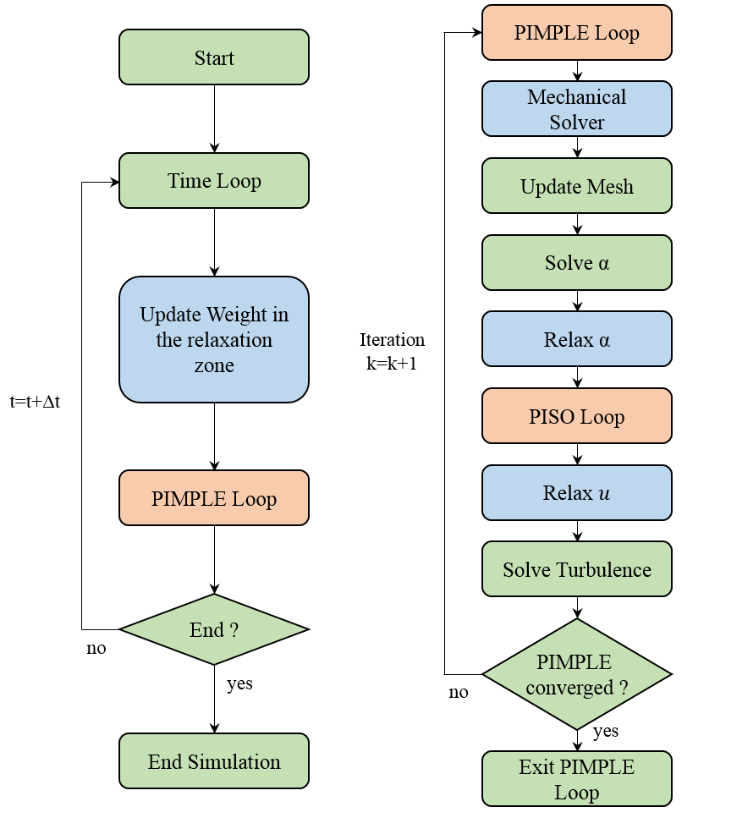
\includegraphics[width=\textwidth]{foamStar.png}
 \caption{Computational algorithm in foamStar(from Monroy et al \cite{Monroy2016})}
 \label{foamStar}
\end{figure}

\section*{SWENSE}
In this section, mathematical model and numerical methods for SWENSE method for two phase solvers is discussed in short. The SWENSE (Spectral Wave Explicit  Navier Stokes Equation) method is proposed to speed up NS solver as mentioned in the functional decomposition technique earlier. This method uses potential wave models to obtain the Incident wave solution efficiently and couples it with viscous solver. Consequently, the viscous solver is only responsible to solve a complementary field (difference from incident wave solution caused by structure and viscosity). The governing equations of the complementary fields are called the Spectral Wave Explicit Navier Stokes Equations (SWENSE). 

\begin{equation}
\chi=\chi_I+\chi_C
\end{equation}
The primary variables (pressure,velocity and free surface elevation) of the flow $\chi$ 
is divided into incident part $\chi_I$ and a complementary part $\chi_C$. The SWENSE method defines this variables in the respective fields as, 

\begin{enumerate}
\item Total field ($\chi$) : It represents the real flow in the computational domain, final solution of the wave structure interaction problem. The flow is governed by in-compressible Navier-Stokes equation
\item Incident field($\chi_I)$:  This part represents the propagation of incident waves in the computational domain without structures. Also the flow is assumed to be irrotational and viscosity of fluid is neglected, so that this part is solved by potential theory with dedicated non linear spectral wave models. This flow is governed by incompressible Euler equations
\item Complementary field ($\chi_C$): This part represents the difference between the total field and the incident field ($\chi_C=\chi-\chi_I$). This field is generated due to the structures and the viscosity of the fluid. The complementary variables are governed by the Spectral Wave Explicit Navier-Stokes Equations (SWENSE) as shown in the next section.  
\end{enumerate}


For the detailed derivation of SWENSE methodology and its equation, it can be refered at Zhaobin thesis\cite{zhaobin_progress}. The PIMPLE algorithm used in the SWENSE solver is given in the Figure \ref{SWENSE_PIMPLE}. The final form of governing equation to be solved in the viscous domain is : 

\subsubsection*{Non conservative two-phase SWENSE: one-fluid form}
Similar to the one-fluid form of two-phase NS equations, the two-phase flow is modeled as a single mixture fluid of both water and air. The non conservative form two phase NS equations and non conservative form Euler equations(modified equation) are used to derive this equation. \\
The continuity equation is, 

\begin{equation}
\nabla \pmb{u_C}=0
\end{equation}

The momentum equation is derived by subtracting the momentum equation of the modified Euler equations from the NS momentum equation. Use the notion of $p_C=p-p_I^*$, the two phase SWENSE momentum equation written with complementary variables and simplifying the equation,

\begin{equation}\label{SWENSE_NCSV}
\frac{\partial \pmb{u_C}}{\partial t}+ \pmb{u_C.\nabla u_I + u. \nabla u_C}= -\frac{\nabla p_C}{\rho} + \frac{\nabla . (\mu (\nabla u_C + \nabla u_C^T))}{\rho}-\frac{p_I}{\rho_I} \frac{\nabla \rho}{\rho}
\end{equation}

\subsubsection*{Conservative two-phase SWENSE: one-fluid form}


\begin{equation}
 \frac{\partial \pmb{\rho u_C}}{\partial t}+\pmb{\nabla.(\rho u u_C)}+\rho u_C \nabla .u_I =-{\nabla p_C} + {\nabla . (\mu (\nabla u + \nabla u^T))}  +\frac{p_I}{\rho_I} {\nabla \rho}  
\end{equation}

For detailed derivation, refer \cite{zhaobin_progress}. The VOF field is not decomposed in SWENSE as boundness of the complementary field is difficult to define, so that total VOF is bounded between 0 and 1. The transport equation of VOF is same as the two-phase NS equations and it reads, 

\begin{equation} \label{SWENSE_VOF}
\frac{\partial \alpha}{\partial t}+ \pmb{u}. \nabla \alpha = 0
\end{equation}

where $\pmb{u=u_I+u_C}$ is the total velocity solution reconstructed by SWENSE ideology.  
\begin{equation}
\rho =\alpha \rho_w+(1-\alpha) \rho_a
\end{equation}

\begin{equation}
\mu=\alpha\mu_w+ (1-\alpha) \mu_a
\end{equation}

\begin{figure}
\centering

\begin{center}
\begin{adjustbox}{width=1.5\textwidth,height=17cm,keepaspectratio}
\begin{tikzpicture}[node distance=2cm]
\centering
\node (start)[startstop]{Start time loop};
\node (c1)[connect, below of=start]{};
\node (pro0) [process0, below of=c1] {Update Incident waves $\pmb{u}_I$ and $p_I$};
\node (in1) [io, right of=pro0, xshift=4cm] {From the Incident wave soltions};


\node (c2)[connect, below of=pro0]{};

\node (pro1) [process0, below of=c2] {Reconstruction $\pmb{u}=\pmb{u}_I+\pmb{u}_C$};
%\filldraw[fill=blue!20!white] (-4,-9) -- (-4,-17.75) -- (10,-17.75) -- (10,-9) node[pos=0.5] {\textbf{PISO loop}};
\node (pro2) [process0, below of=pro1] {Solve for $\alpha$ (Eqn.(\ref{SWENSE_VOF}))};
\node (pro3) [process, below of=pro2] {Update $\rho,\mu$ and $p_I^*$};


%\filldraw[fill=red!20!white, opacity =0.3] (-6,-5) -- (-6,-22) -- (13,-22) -- (13,-5) node[pos=0.5] {\textbf{PIMPLE loop}};

\node (pro4) [process0, right of=pro3, xshift=5cm] {Start $u_C -p_C$ coupling (PISO)};
\node (pro5) [process0, below of=pro4] {Solve for $\pmb{u}_C$};
\node (pro6) [process0, below of=pro5] {Solve for $p_C$};
\node (pro7) [process0, below of=pro6] {Update velocity $\pmb{u}_C$};
\node (dec0) [decision, below of=pro7, yshift=-1 cm] {PISO Convergence?};
\node (pro8) [process, left of=dec0, xshift=-5cm] {Relaxation zones};
\node (dec1) [decision, below of=pro8, yshift=-2 cm] {PIMPLE Convergence?};
\node (dec2) [decision, right of=dec1, xshift=5 cm] {$t+\Delta t \ge T$};
\node (stop)[startstop, below of=dec2, yshift=-2 cm]{End time loop};

\draw [arrow] (start) -- node[anchor=east] {t=0} (c1);
\draw [arrow] (c1) -- (pro0);
\draw [arrow](in1) -- (pro0.east);
\draw [arrow] (pro0) -- node[anchor=east] {PIMPLE iter=0} (c2);
\draw [arrow] (c2) -- node[anchor=east] {PIMPLE iter +=1}(pro1);
\draw [arrow] (pro1) -- (pro2);
\draw [arrow] (pro2) -- (pro3);
\draw [arrow] (pro3) -- (pro4);
\draw [arrow] (pro4) -- (pro5);
\draw [arrow] (pro5) -- (pro6);
\draw [arrow] (pro6) -- (pro7);
\draw [arrow] (pro7) -- (dec0);
\draw [arrow] (dec0) -- node[anchor=north] {Yes} (pro8);

\draw [arrow](dec0.east) node[anchor=south] {No} -- ++(2cm,0) |- (pro6.east);
\draw [arrow] (pro8) -- (dec1);
\draw [arrow](dec1.west) node[anchor=north] {No} -- ++(-3cm,0) |- (c2.west);

\draw [arrow] (dec1) -- node[anchor=north] {Yes} (dec2);

\draw [arrow](dec2.east) node[anchor=north] {No} -- ++(3cm,0) |-  (c1.east);
\draw [arrow] (dec2) -- node[anchor=east] {Yes} (stop);

\end{tikzpicture}
\end{adjustbox}

\end{center}
\caption{Figure: PIMPLE algorithm in SWENSE method }
\label{SWENSE_PIMPLE}
\end{figure}

\section{Validation of solvers}
\textbf{Wave only validation}: Different wave only cases like regular waves, irregular waves and focusing waves were generated from potential domain(HOS-NWT) and it is coupled with the both the foamStar and SWENSE solvers using Grid2Grid wrapper program developed by Choi et al \cite{Choi2017}. The results were used to parametric the needed information for 3D Mesh for next sections. Validation results are not given here but the results were observed to be within the error of less than 1 \% . \\
\textbf{Wave structure validation} : Figure \ref{foamStar_validation}.  shows the different test cases carried out in foamStar for 3D wave structure validation in relation to experiments and complex wave generation . For more details related to experiment considered refer with Sriram et al \cite{SRIRAM2015279},\cite{sriramexpt}, Arndt et al \cite{hilderbrandtexpt}
\begin{figure}
 \centering 
 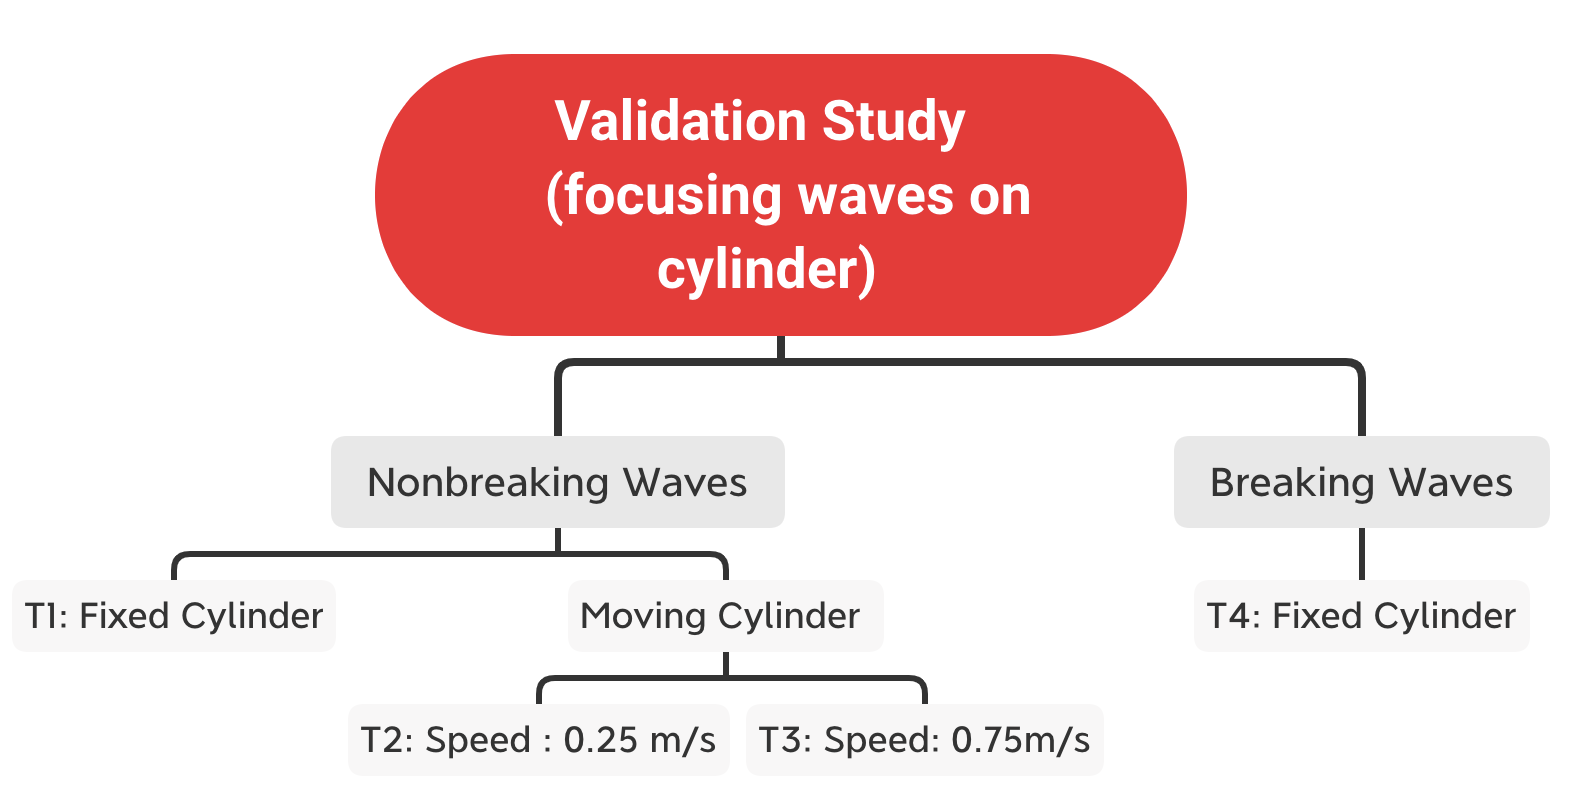
\includegraphics[width=\textwidth]{foamStar_testcase.png}
 \caption{Test cases of foamStar Validation}
 \label{foamStar_validation}
\end{figure}

All the testcases mentioned were  validated and submitted the results for publication in IJOPE(2020). One of the test case, non breaking focusing waves on the fixed cylinder is shown here as the preliminary study. 

\subsection{Numerical set up and parameters}
The nonbreaking focusing wave for this test case is generated by the time reversal technique \cite{Ducrozet2019}.  Other input details for potential wave generation in the HOS NWT are as mentioned in the Table \ref{tab:HOS_input}. There are 7 probes placed in the towing tank and the wave generated in the HOS-NWT is compared with the experimental probe details to confirm the accuracy of the wave. The probe details of HOS match well with experimental wave probes, confirming its accuracy.  
\begin{table}[]
\centering
\begin{tabular}{l|c}
\multicolumn{1}{c|}{\textbf{Parameters}}                                  & \textbf{Values}                   \\ \hline
Tank Dimensions                                                           & 50 X 2.2 X 0.7                    \\
Low cut off freq(Hz)                                                      & 0.3                               \\
High cut off freq(Hz)                                                     & 3                                 \\
Order of wavemaker                                                        & 2                                 \\
wave maker type                                                           & Hinged                            \\
Rotational axis distance                                                  & 0 \\
Time ramp duration                                                        & 1                                 \\
Beginning of beach                                                        & 0.8                               \\
Absorption strength                                                       & 1                                 \\
Duration of simulation                                                    & 50 \\
Time tolerance                                                            & 1.e-7                   \\
Output frequency                                                          & 30                                \\
Order of HOS                                                              & 5                                 \\
SWENSE output                                                             & 1                                 \\
\begin{tabular}[c]{@{}l@{}}Probes location from\\ Wave maker\end{tabular} & \multicolumn{1}{l}{4.975m,13.928m,14.178m,14.428m,24.31m,24.88m,25.585m}

\end{tabular}

\caption{Input details for focusing wave generation in HOS NWT}
\label{tab:HOS_input}
\end{table}

\begin{figure} []
    \centering
    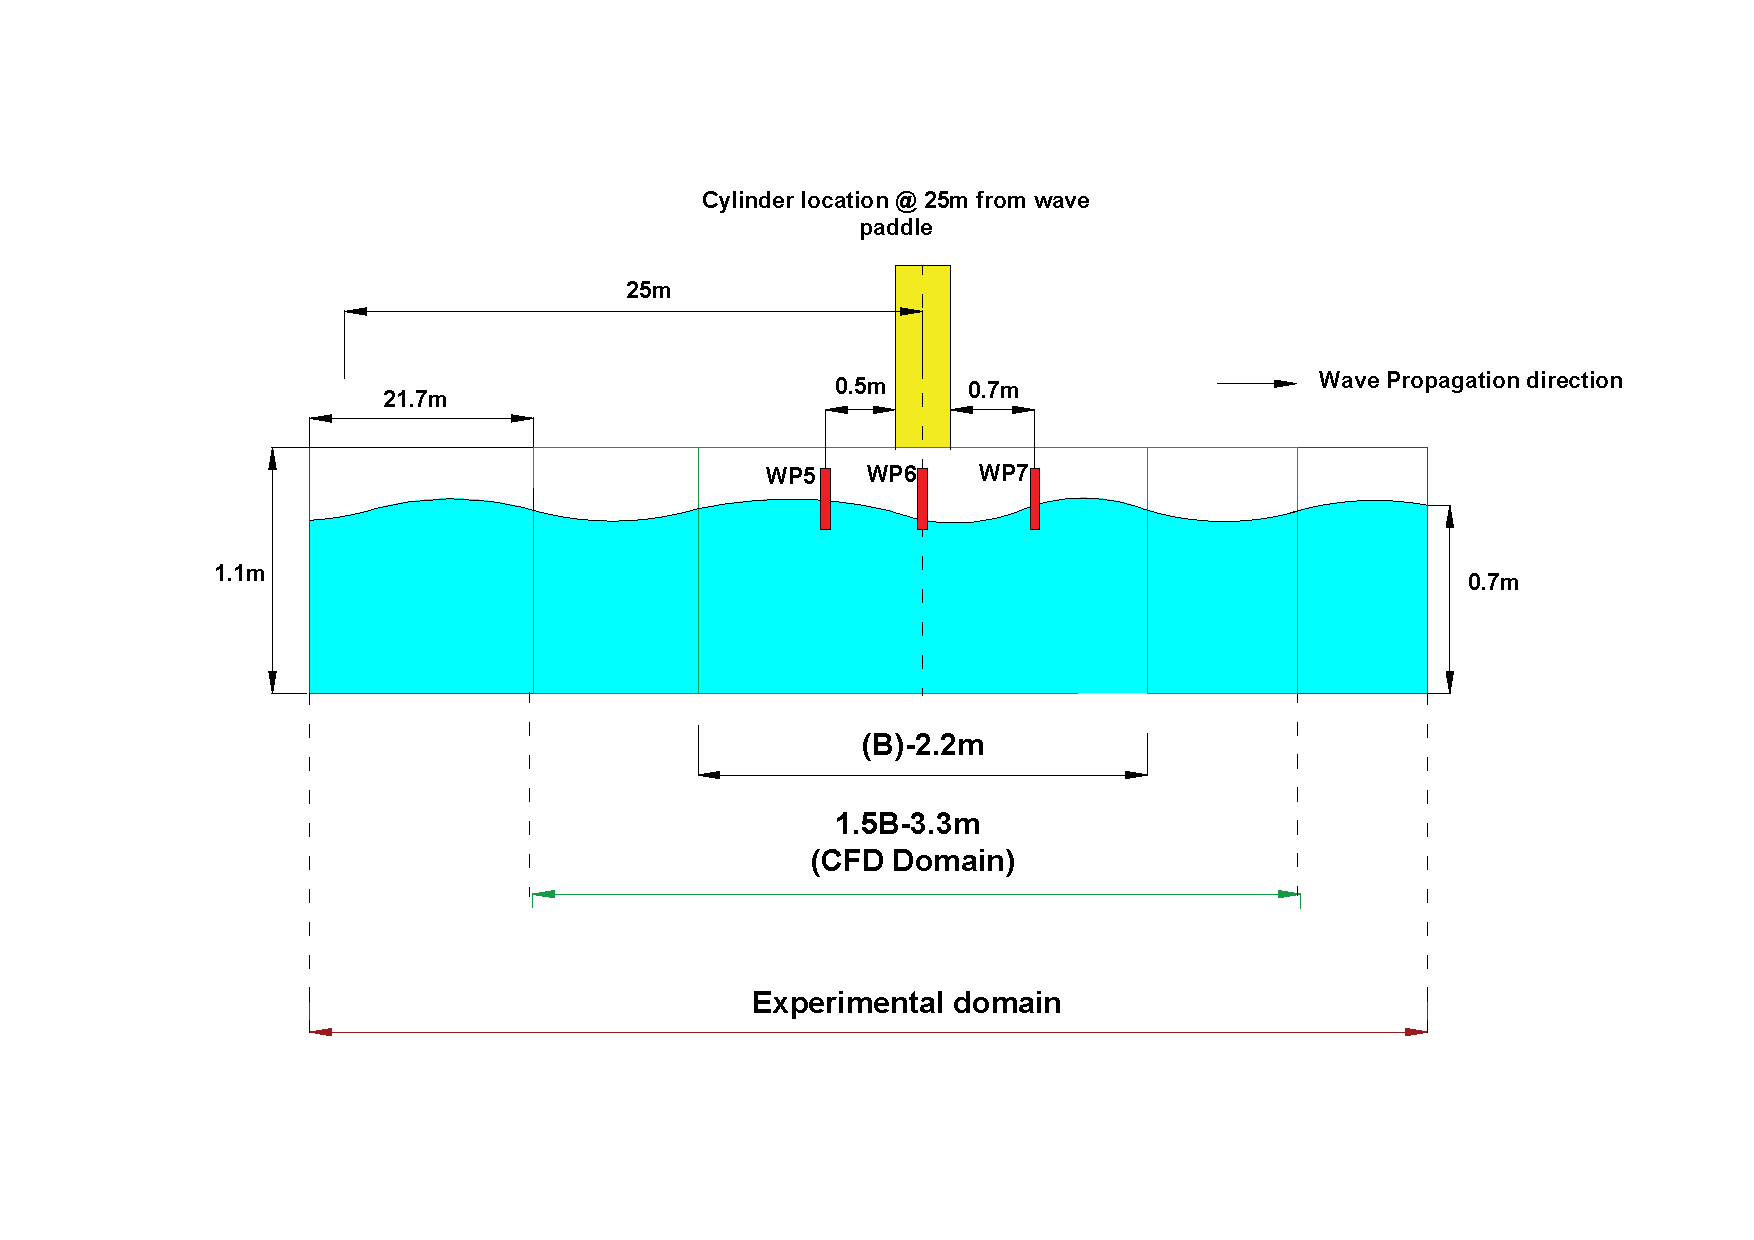
\includegraphics[width=\textwidth,height=0.4\textheight]{Wave_probe_location_cropped.pdf}
    \caption{Wave probe location in the computational and experimental domain to be compared with their nomenclature and their exact location}
    \label{fig:WP_location}
\end{figure}
\begin{figure} []
    \centering
    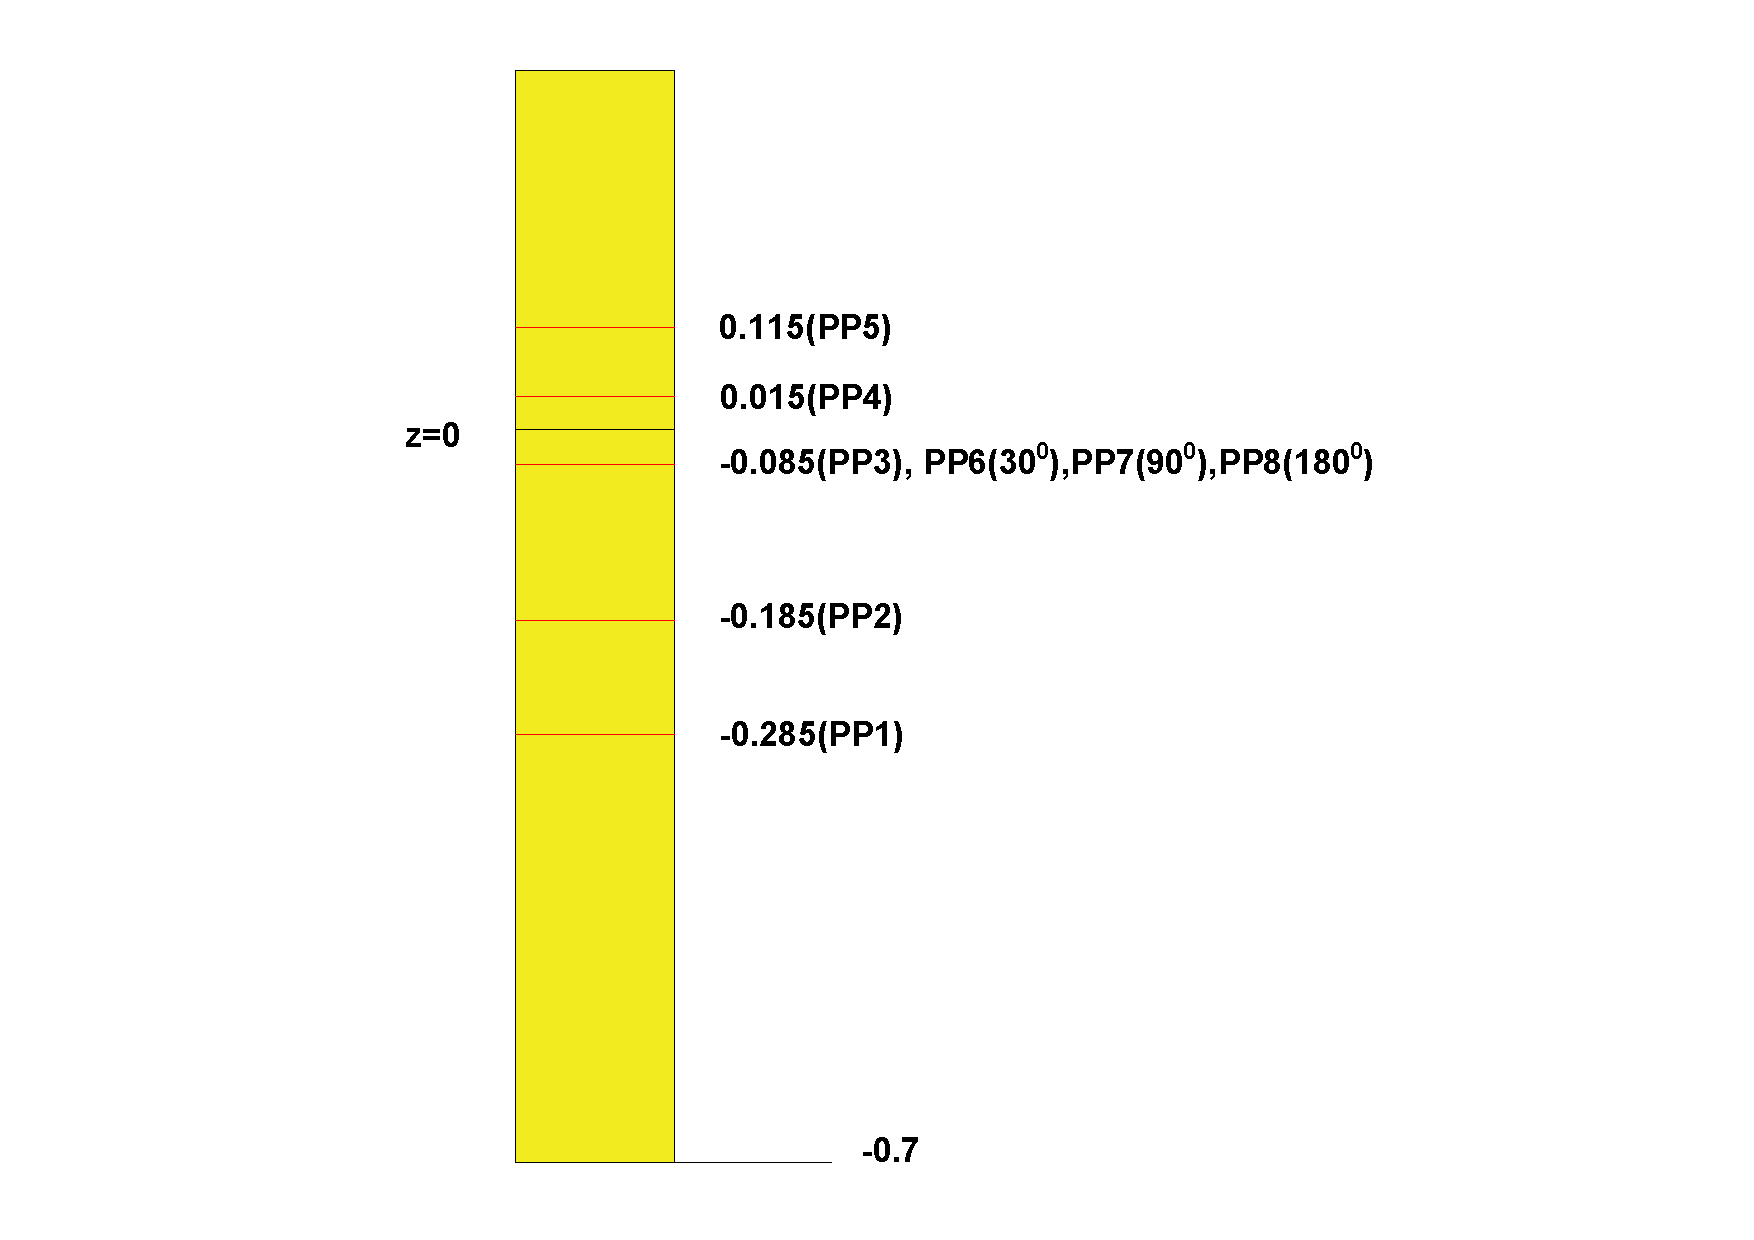
\includegraphics[width=0.5\textwidth,height=0.4\textheight]{Pressure_probe_location_cropped.pdf}
    \caption{Pressure probe location on the cylinder in the computational domain and experimental domain with their nomenclature}
    \label{fig:PP_location}
\end{figure}

\subsection{Comparison with experimental results}
In generic description, CFD domain is placed inside the HOS domain as shown in the Figure \ref{fig:WP_location}. To replicate the experiment carried out for this case the cylinder of diameter 0.22m is chosen and placed with wave probes as shown in the Figure \ref{fig:WP_location}. Also, to measure the pressure over the cylinder pressure sensors are placed along the length of the cylinder as shown in the Figure \ref{fig:PP_location}. The wave in foamStar is generated using coupling strategy with HOS solver with Grid2Grid a wrapper program\cite{choi_relaxation}. The comparison between numerical and the experimental data are as shown in the figures, Figure \ref{fig:NBR_fixed_WP} and Figure \ref{fig:NBR_fixed_PP}. Only the time window of 3s around the focusing time is shown for better understanding. The time history of wave surface elevation recorded by the wave probe in the CFD domain and experimental domain are shown in the Figure \ref{fig:NBR_fixed_WP}. It is observed that numerical wave surface elevation are as similar to that of experimental wave which in turn makes the pressure time history looks similar as shown in the Figure \ref{fig:NBR_fixed_PP}. Although the amplitude of waves and pressure are in good agreement, still there is a phase shift of 0.1s, reason is yet to be finalized. 
This study hence validated for the performance of foamStar for solving complex wave structure interaction phenomenon. 

	\begin{figure}[H]
	\centering     %%% not \center
    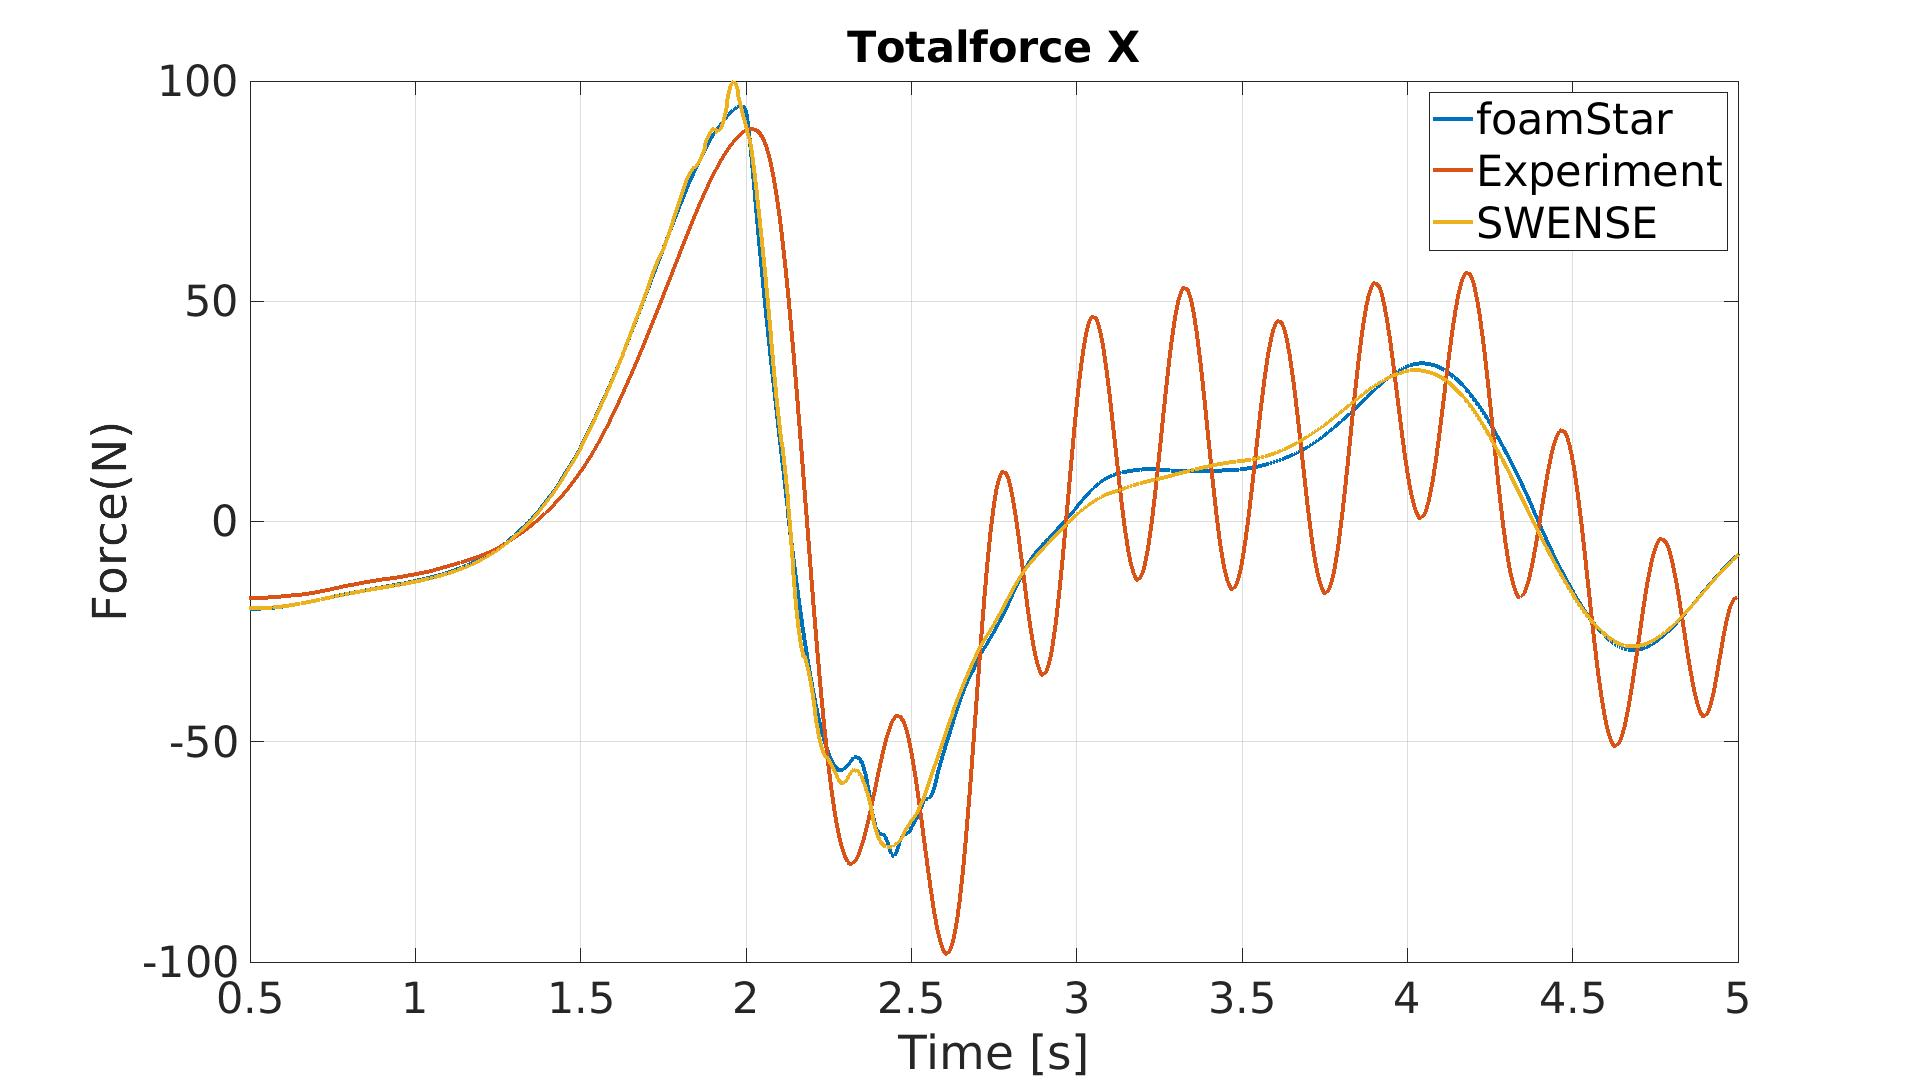
\includegraphics[width=\textwidth]{TotalForce.jpg}
	\caption{Force comparison between numerical and experiment data of the non breaking focusing wave on fixed cylinder }
\end{figure}





\begin{figure}
\centering

\subfloat{%
  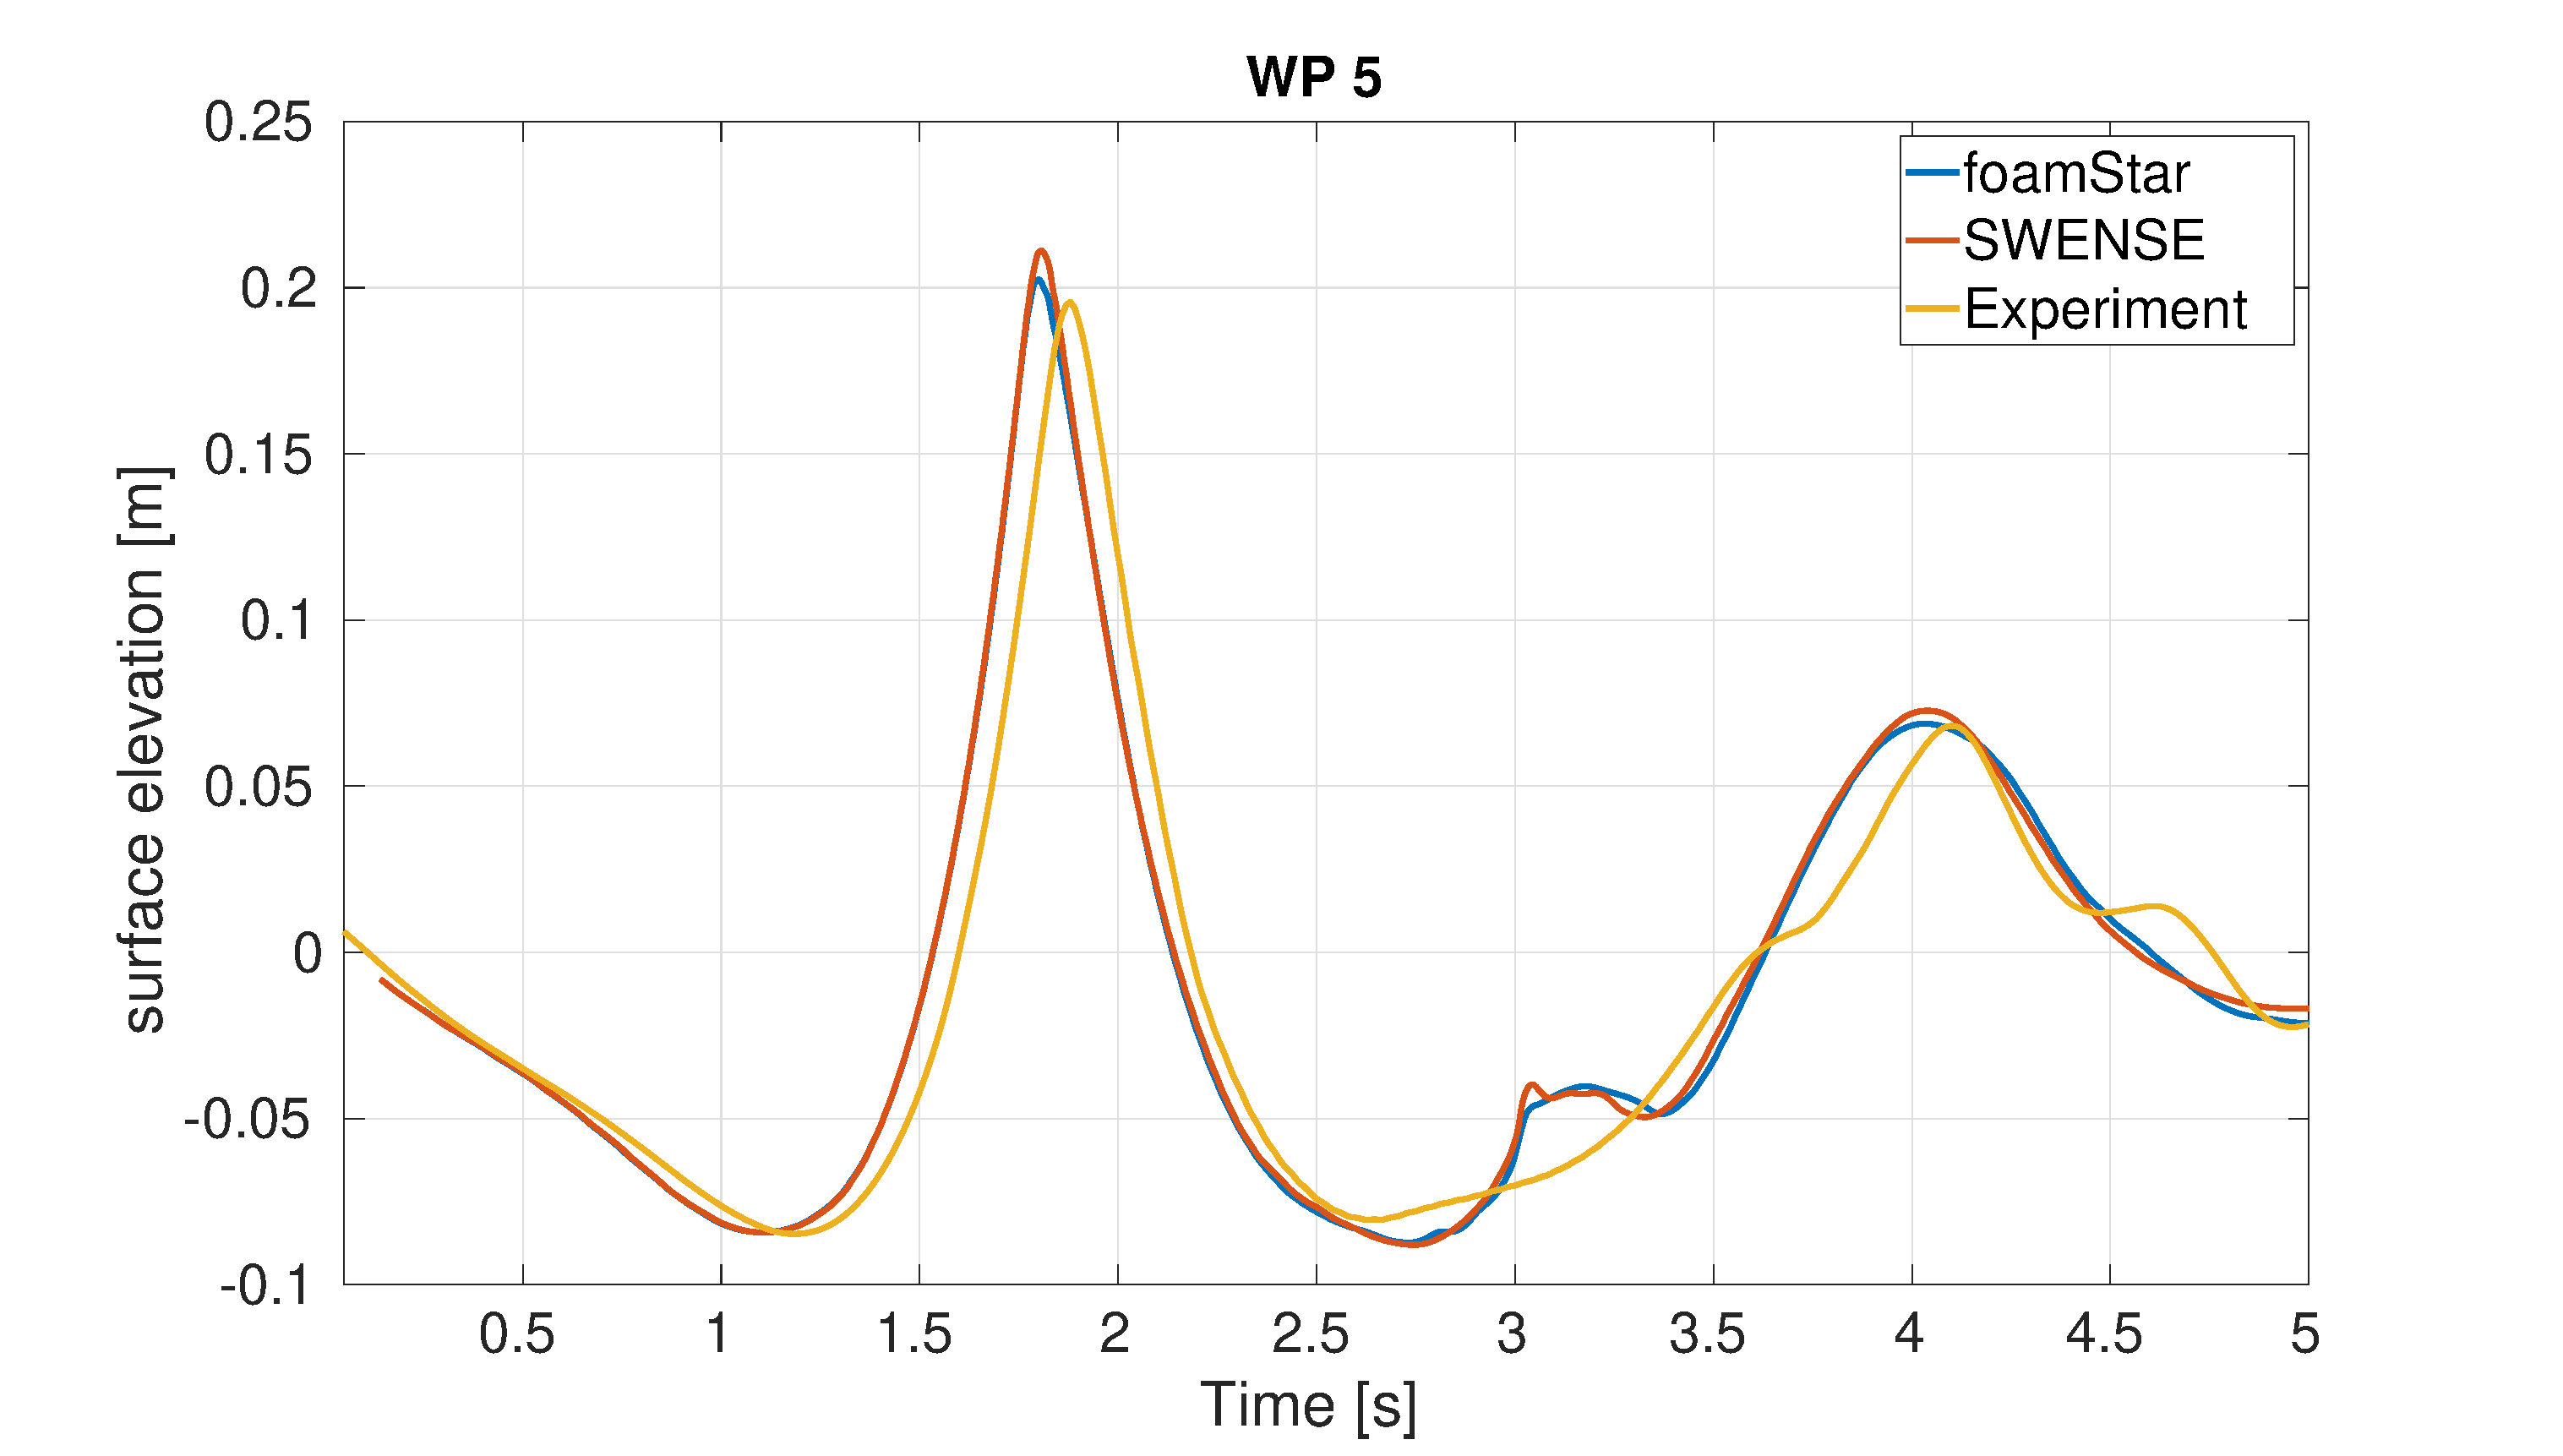
\includegraphics[clip,width=0.85\columnwidth,height=0.275\textheight]{WP5.eps}%
}

\subfloat{%
  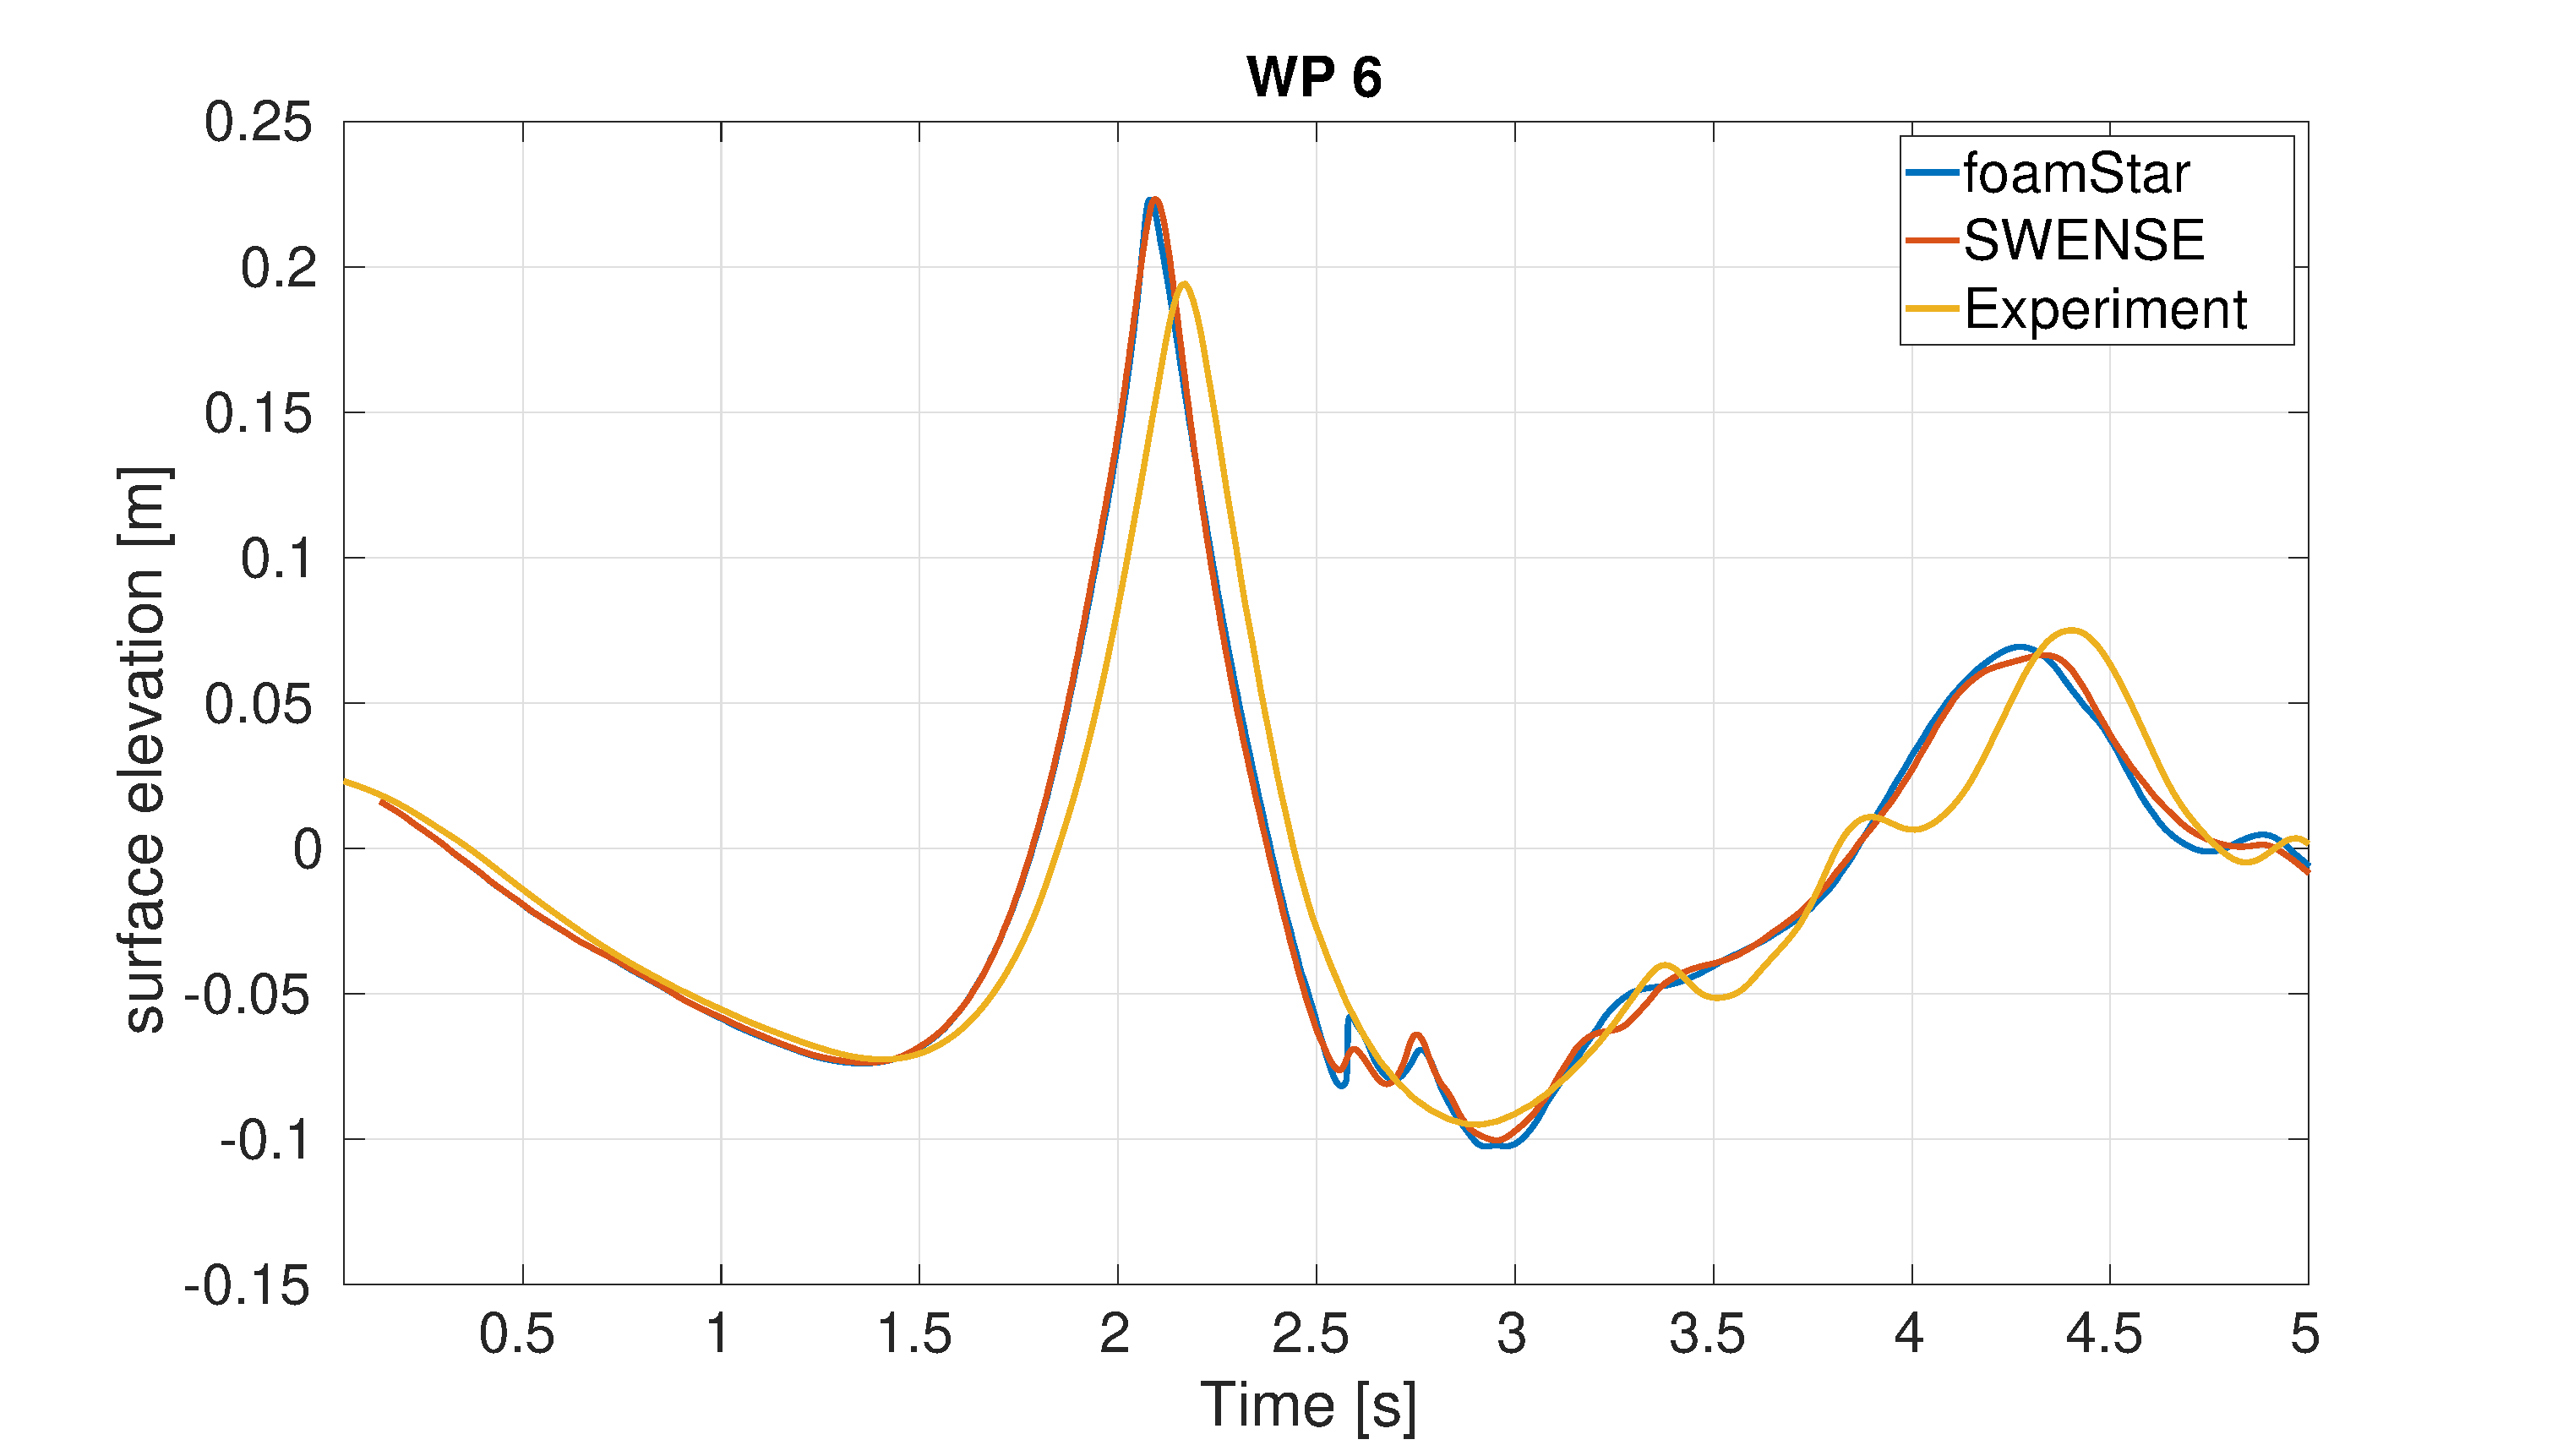
\includegraphics[clip,width=0.85\columnwidth,height=0.275\textheight]{WP6.eps}%
}

\subfloat{%
  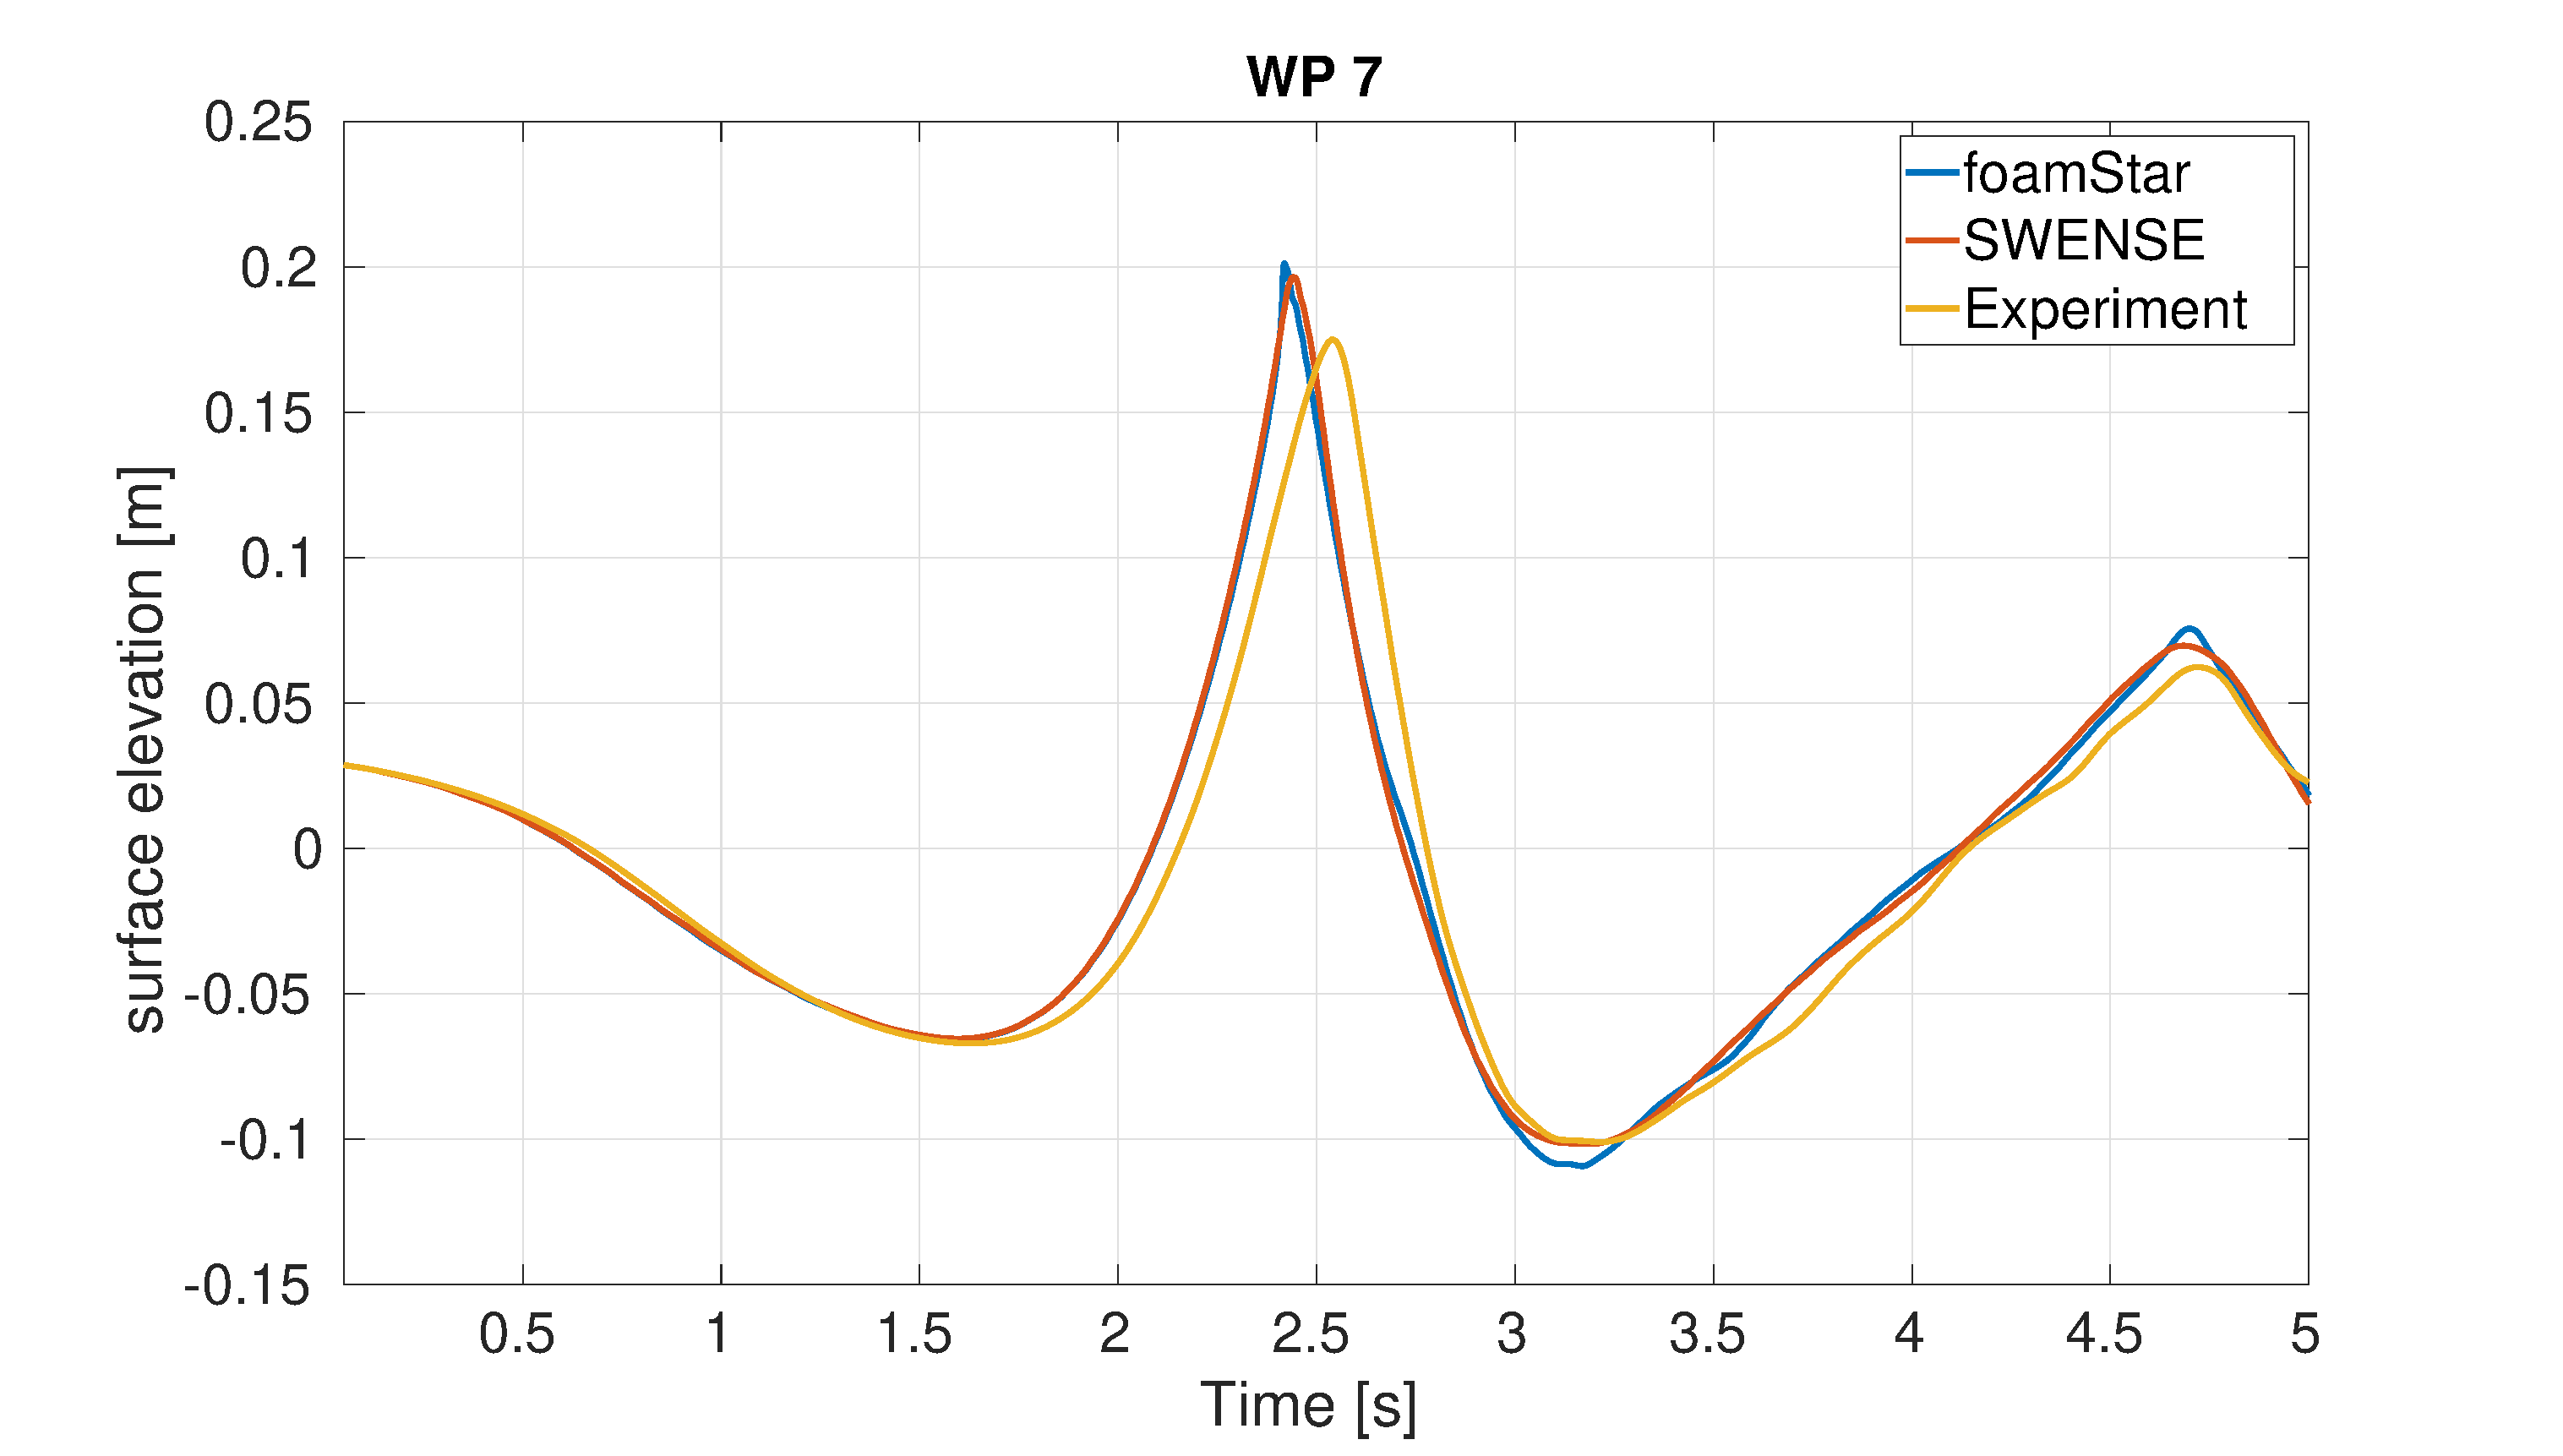
\includegraphics[clip,width=0.85\columnwidth,height=0.275\textheight]{WP7.eps}%
}

\caption{Surface elevation comparison between probes of numerical and experiment data in front,inline and back of the focusing location(cylinder) at focusing time} \label{fig:NBR_fixed_WP}

\end{figure}





\begin{figure}
	\centering
	\captionsetup{justification=centering}
    %%% not \center
	\subfigure[PP2]{\label{Heave_comp1}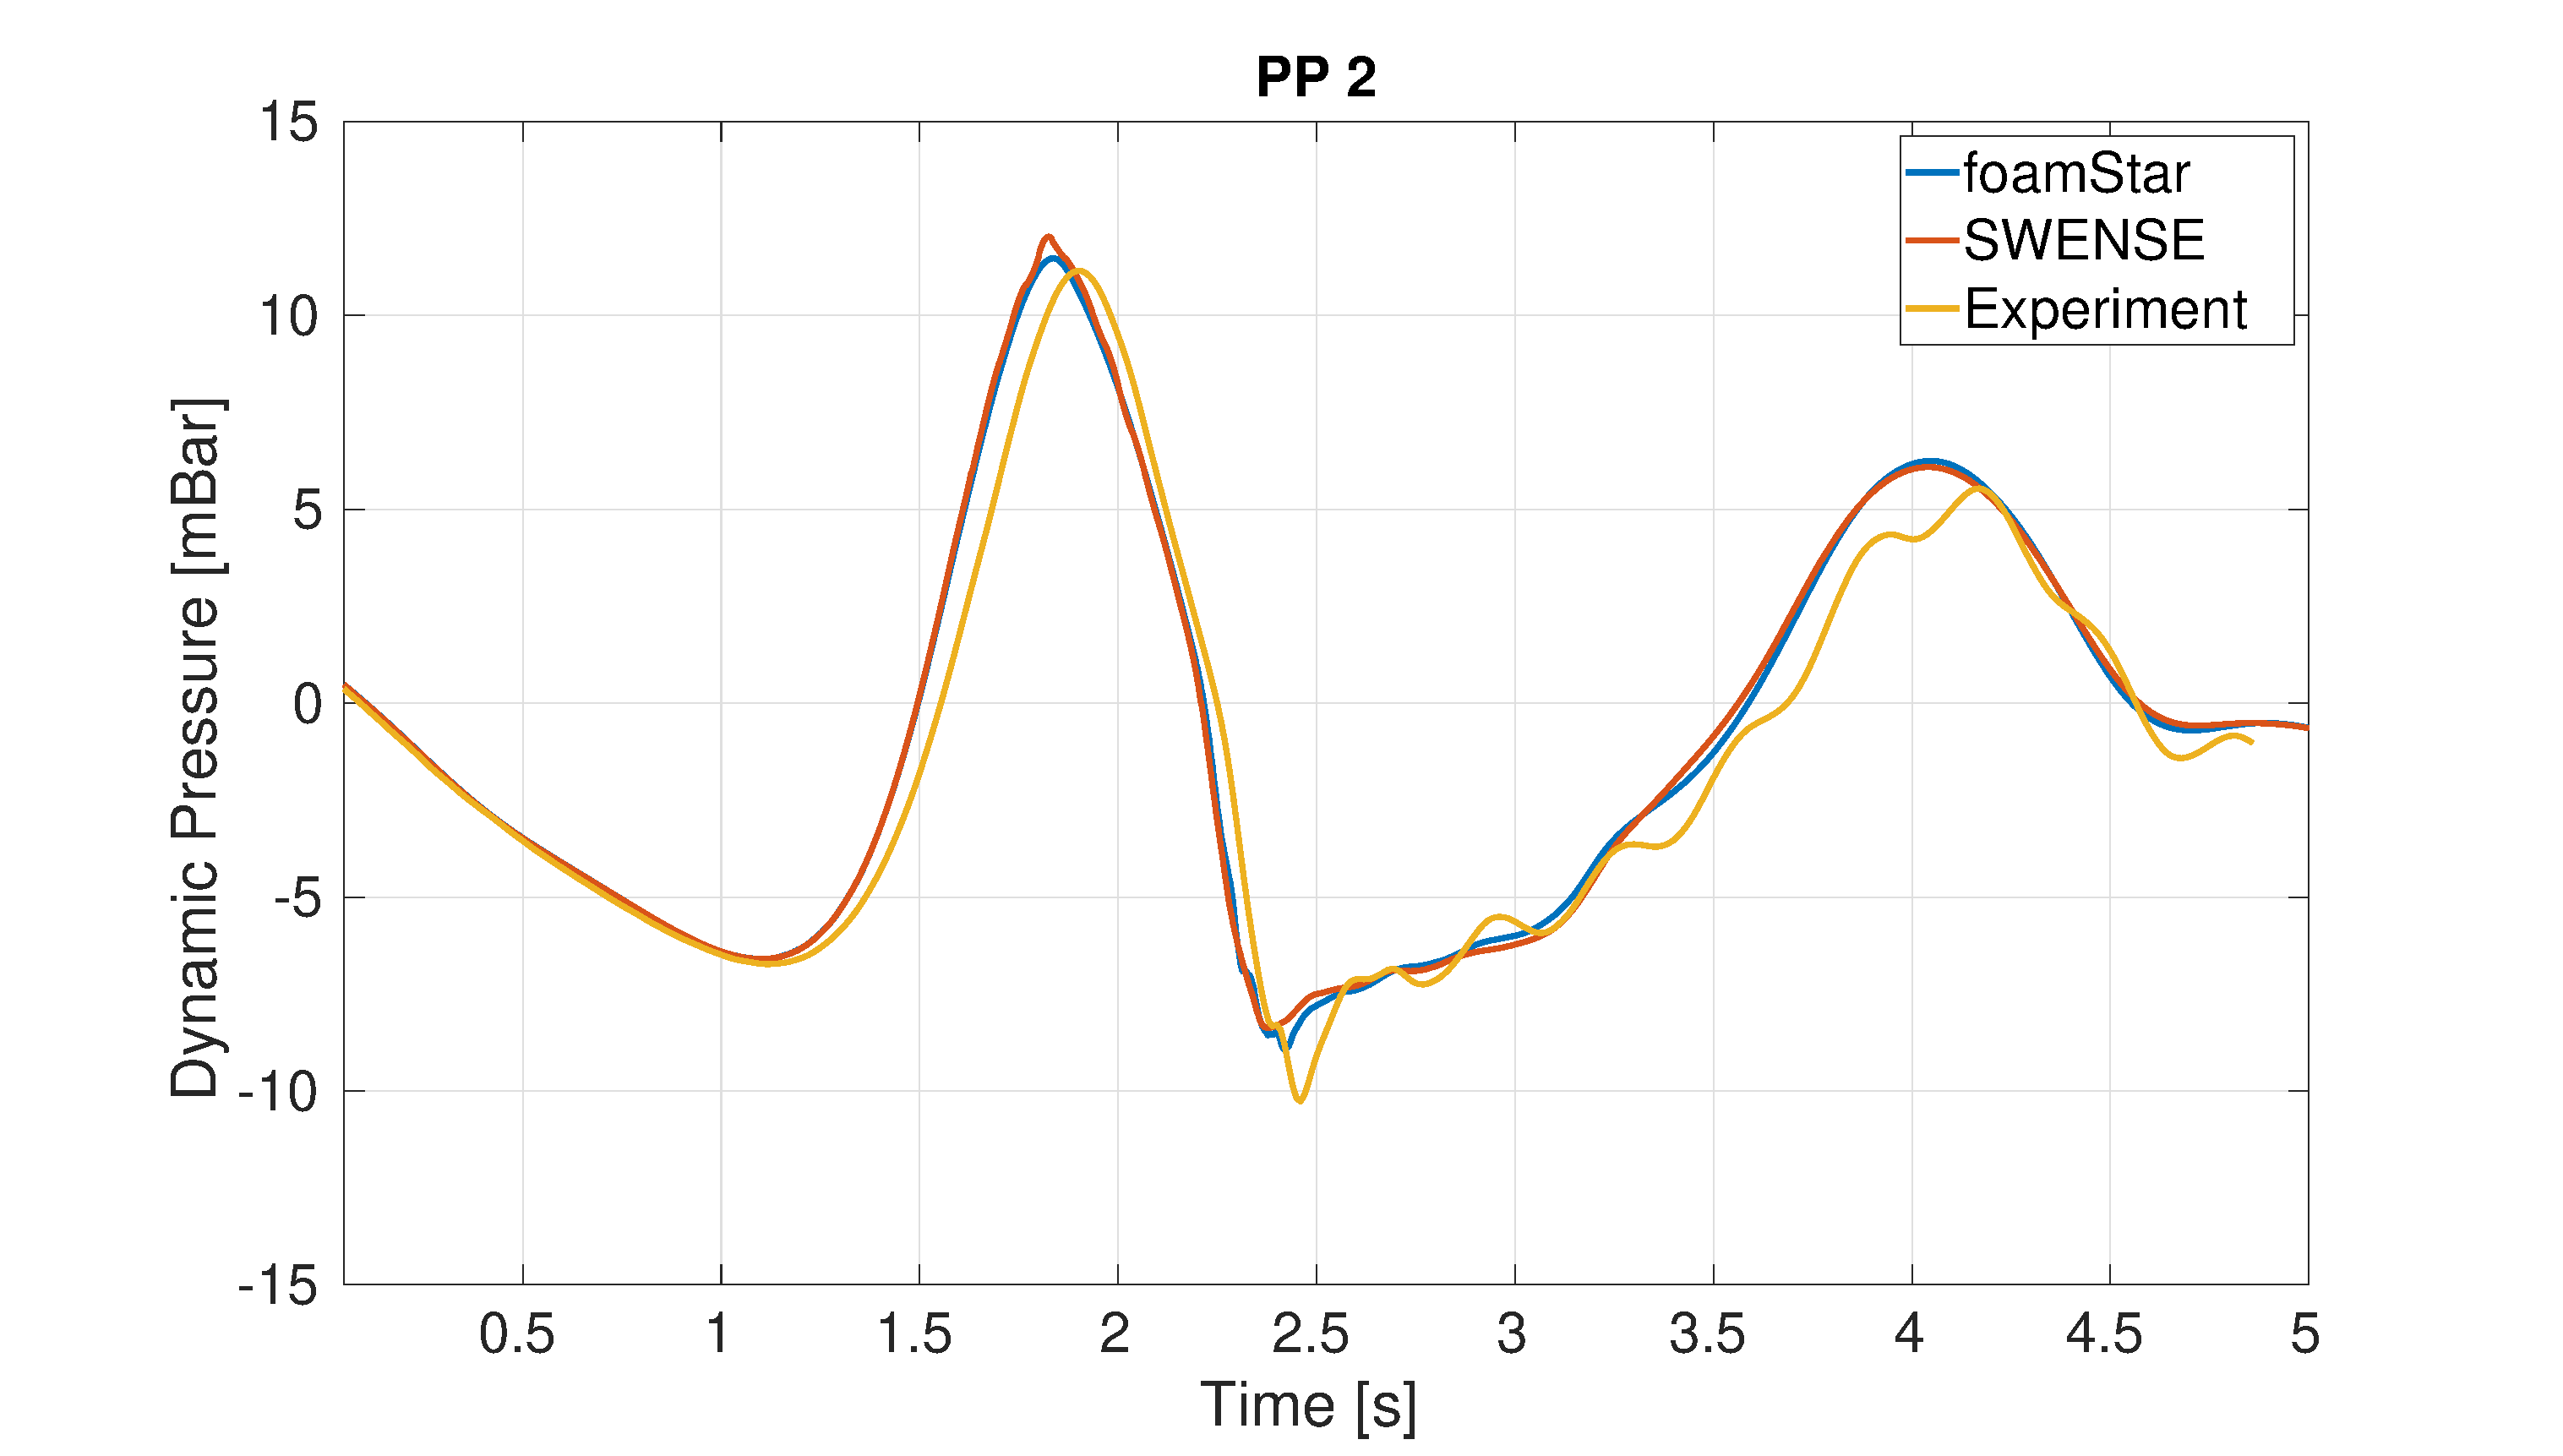
\includegraphics[width=65mm,height=50mm]{PP2.eps}}
    	\subfigure[PP3]{\label{Heave_comp2}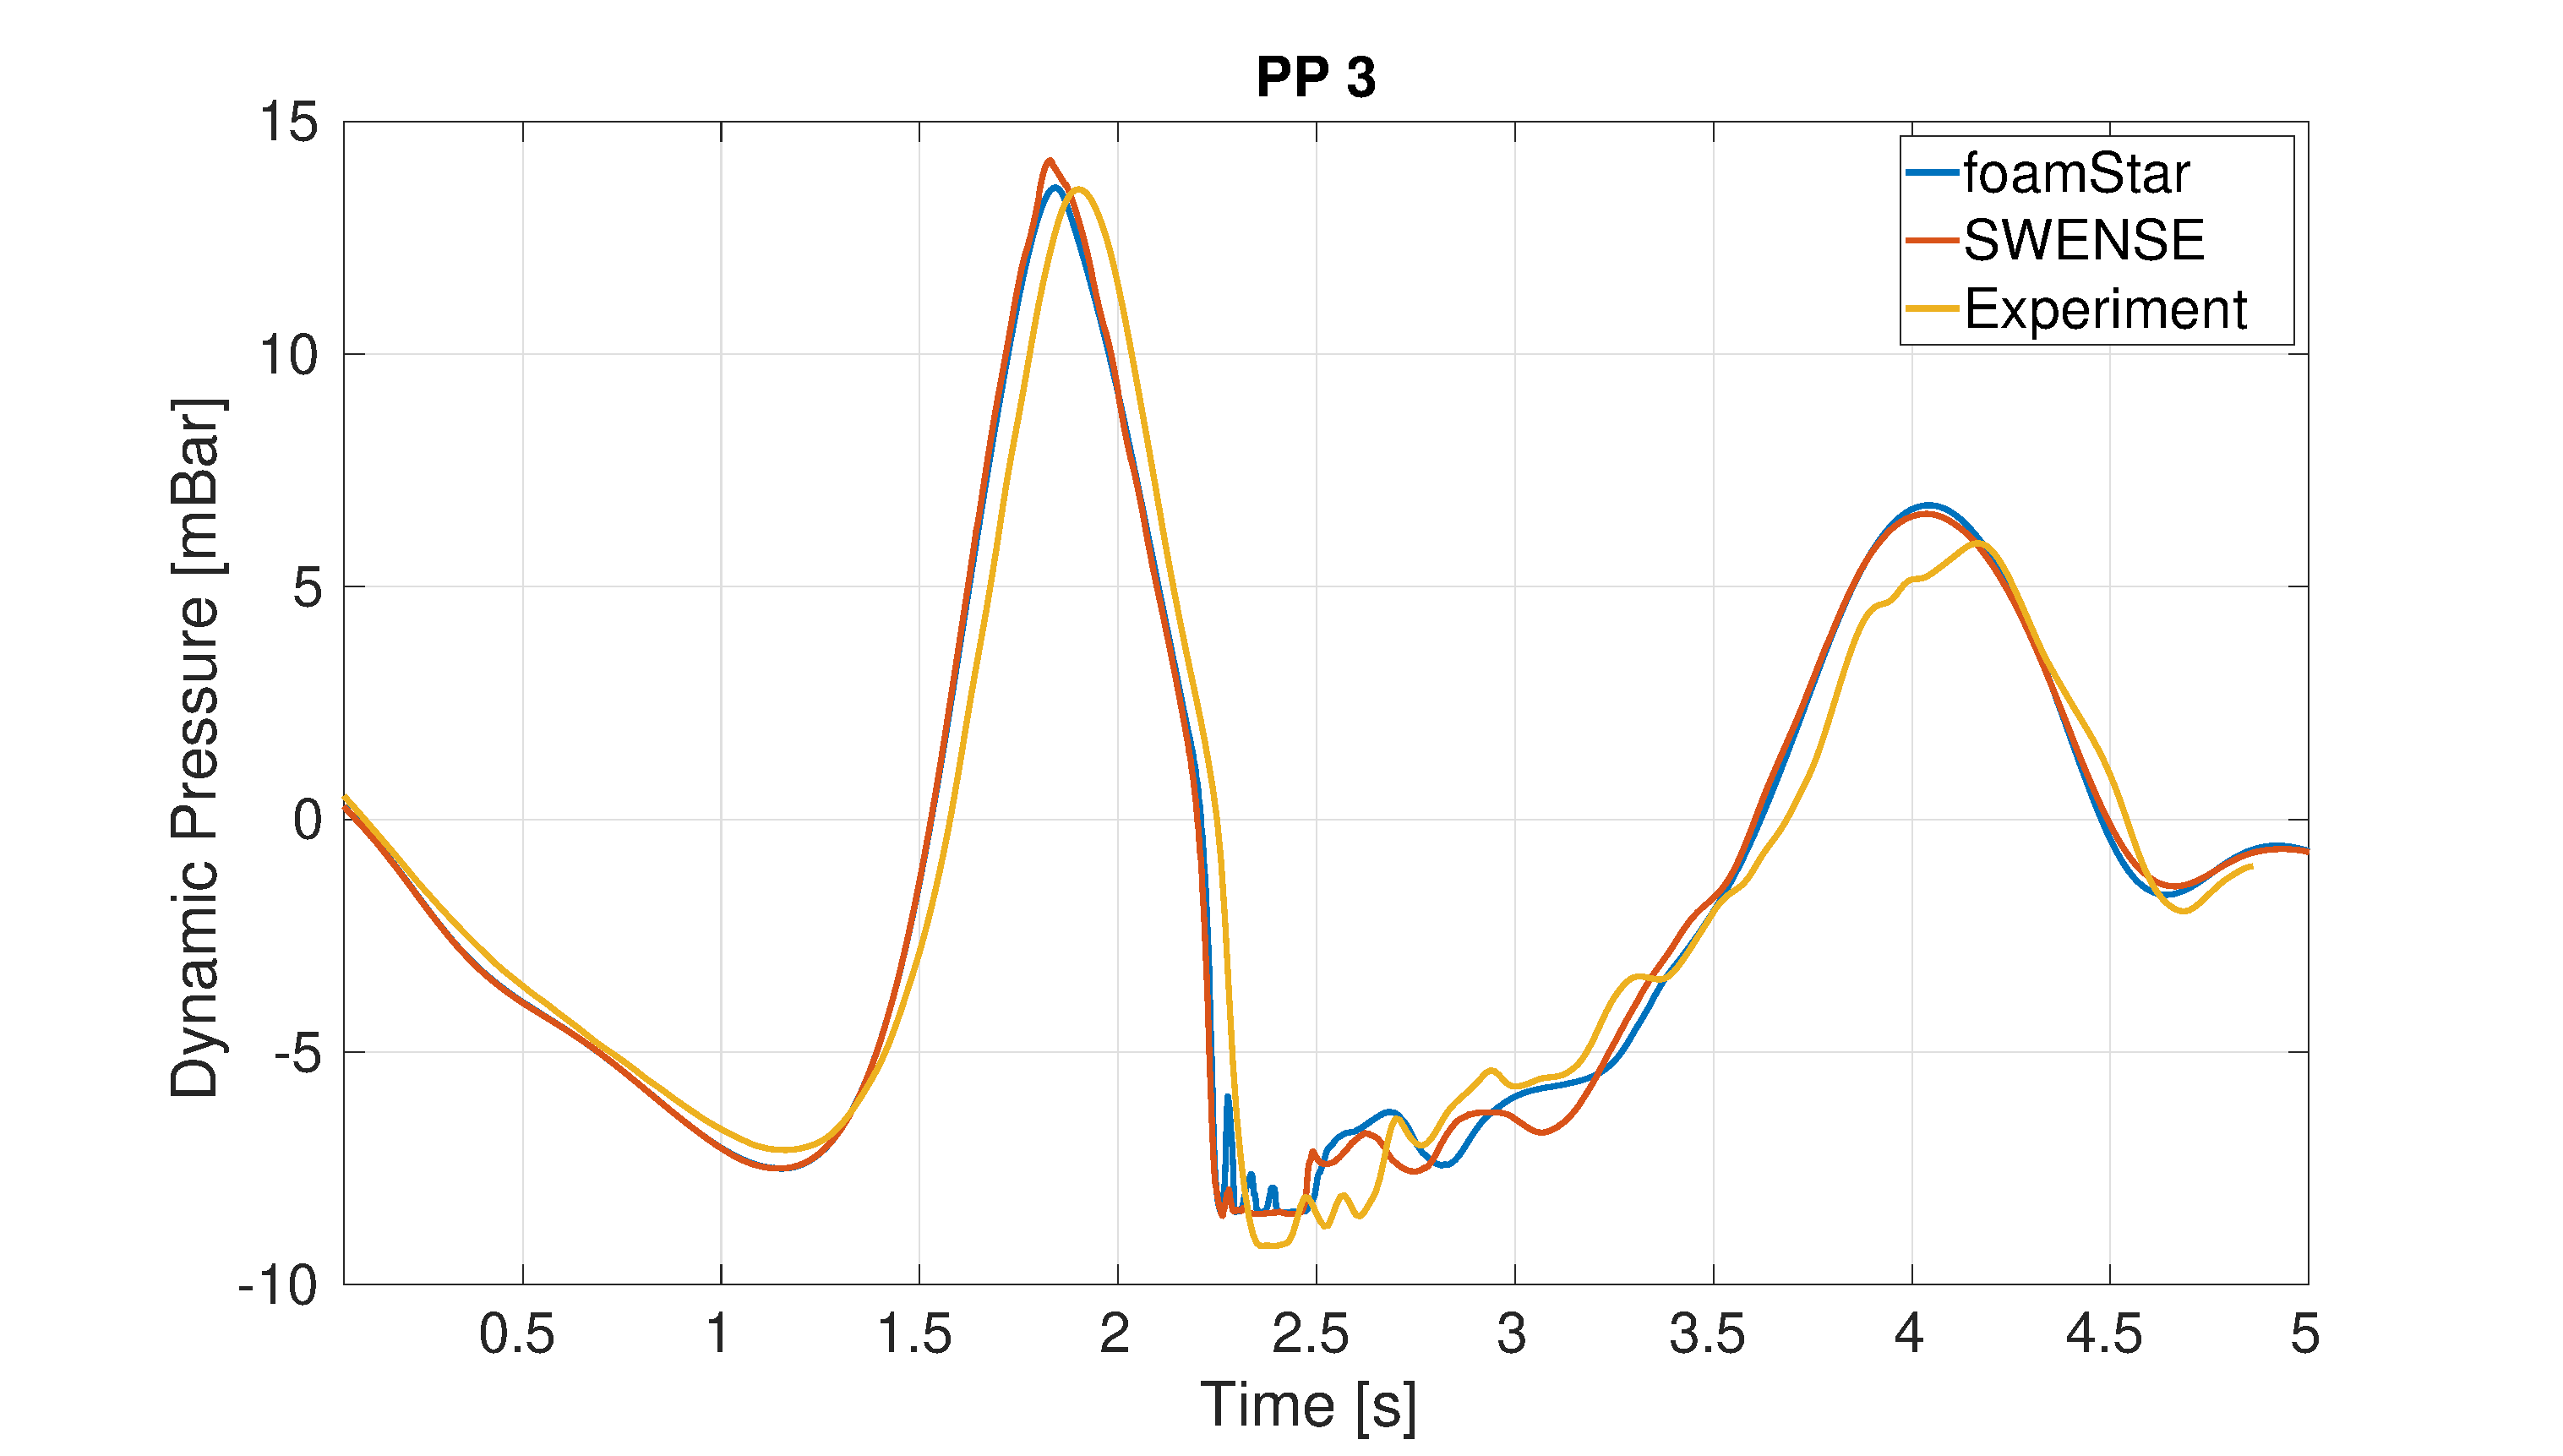
\includegraphics[width=65mm,height=50mm]{PP3.eps}}
        \subfigure[PP4]{\label{Pitch_comp}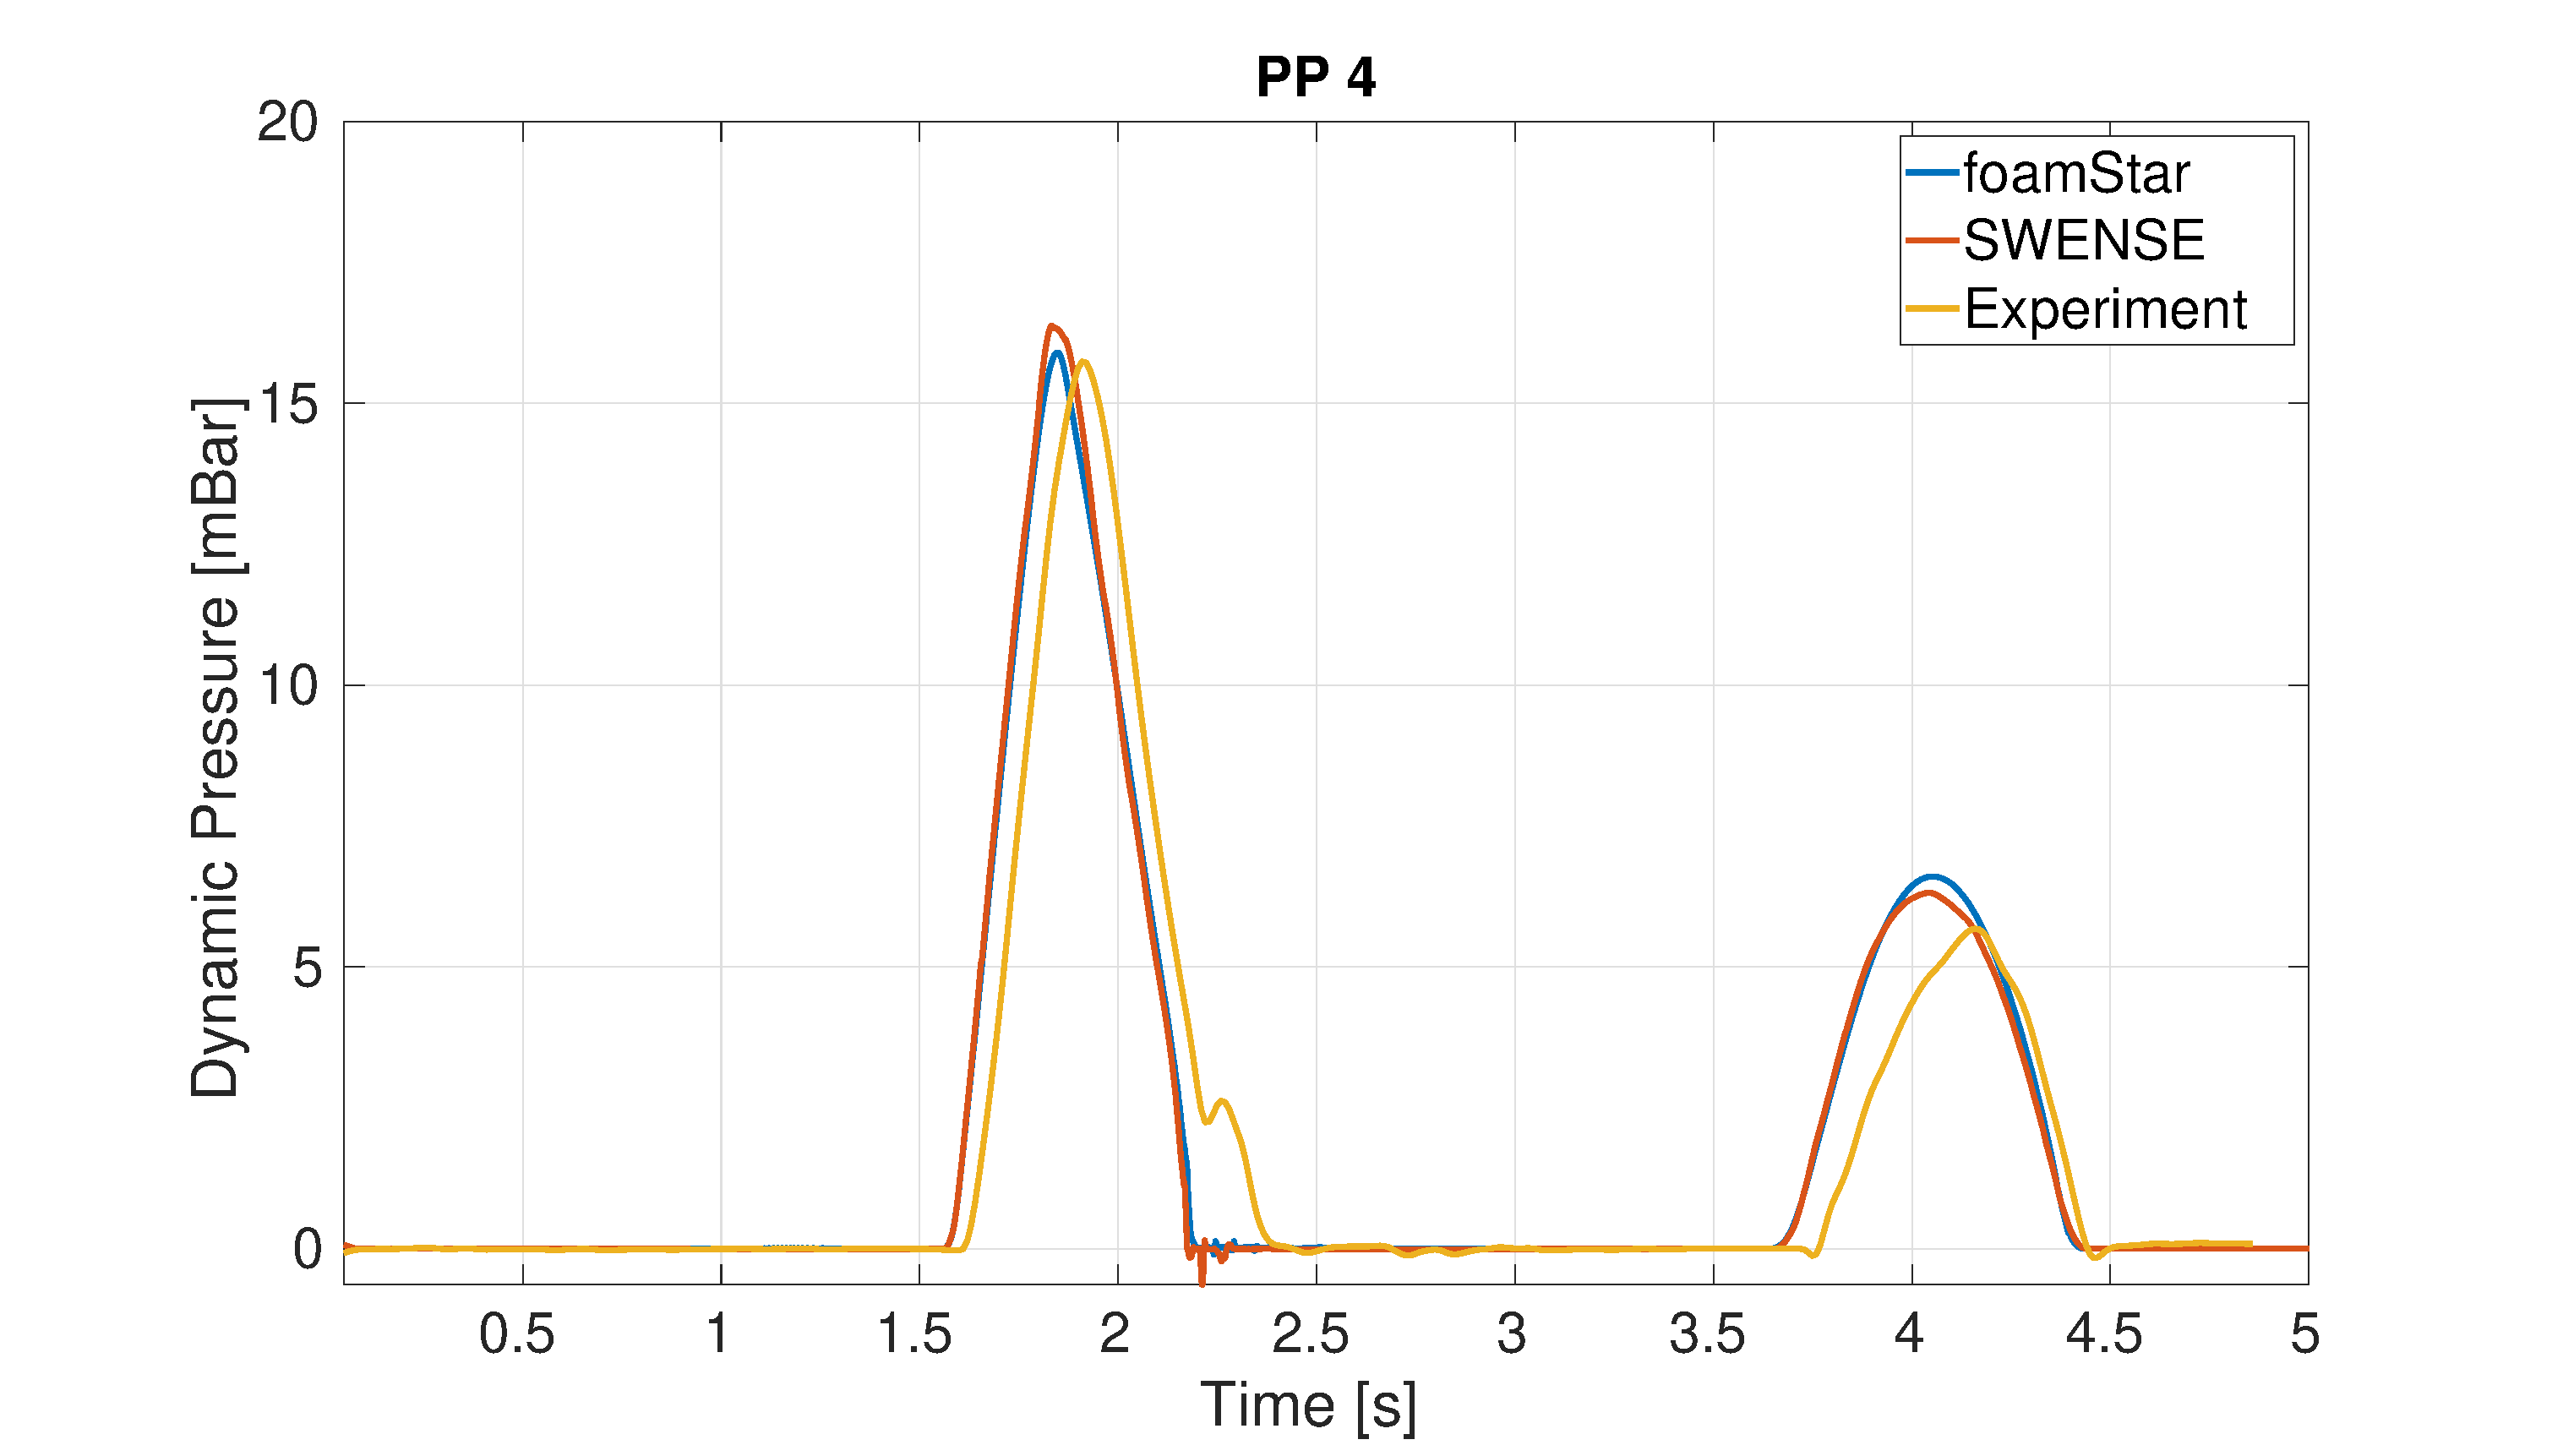
\includegraphics[width=65mm,height=50mm]{PP4.eps}}
	\subfigure[PP5]{\label{Roll_comp}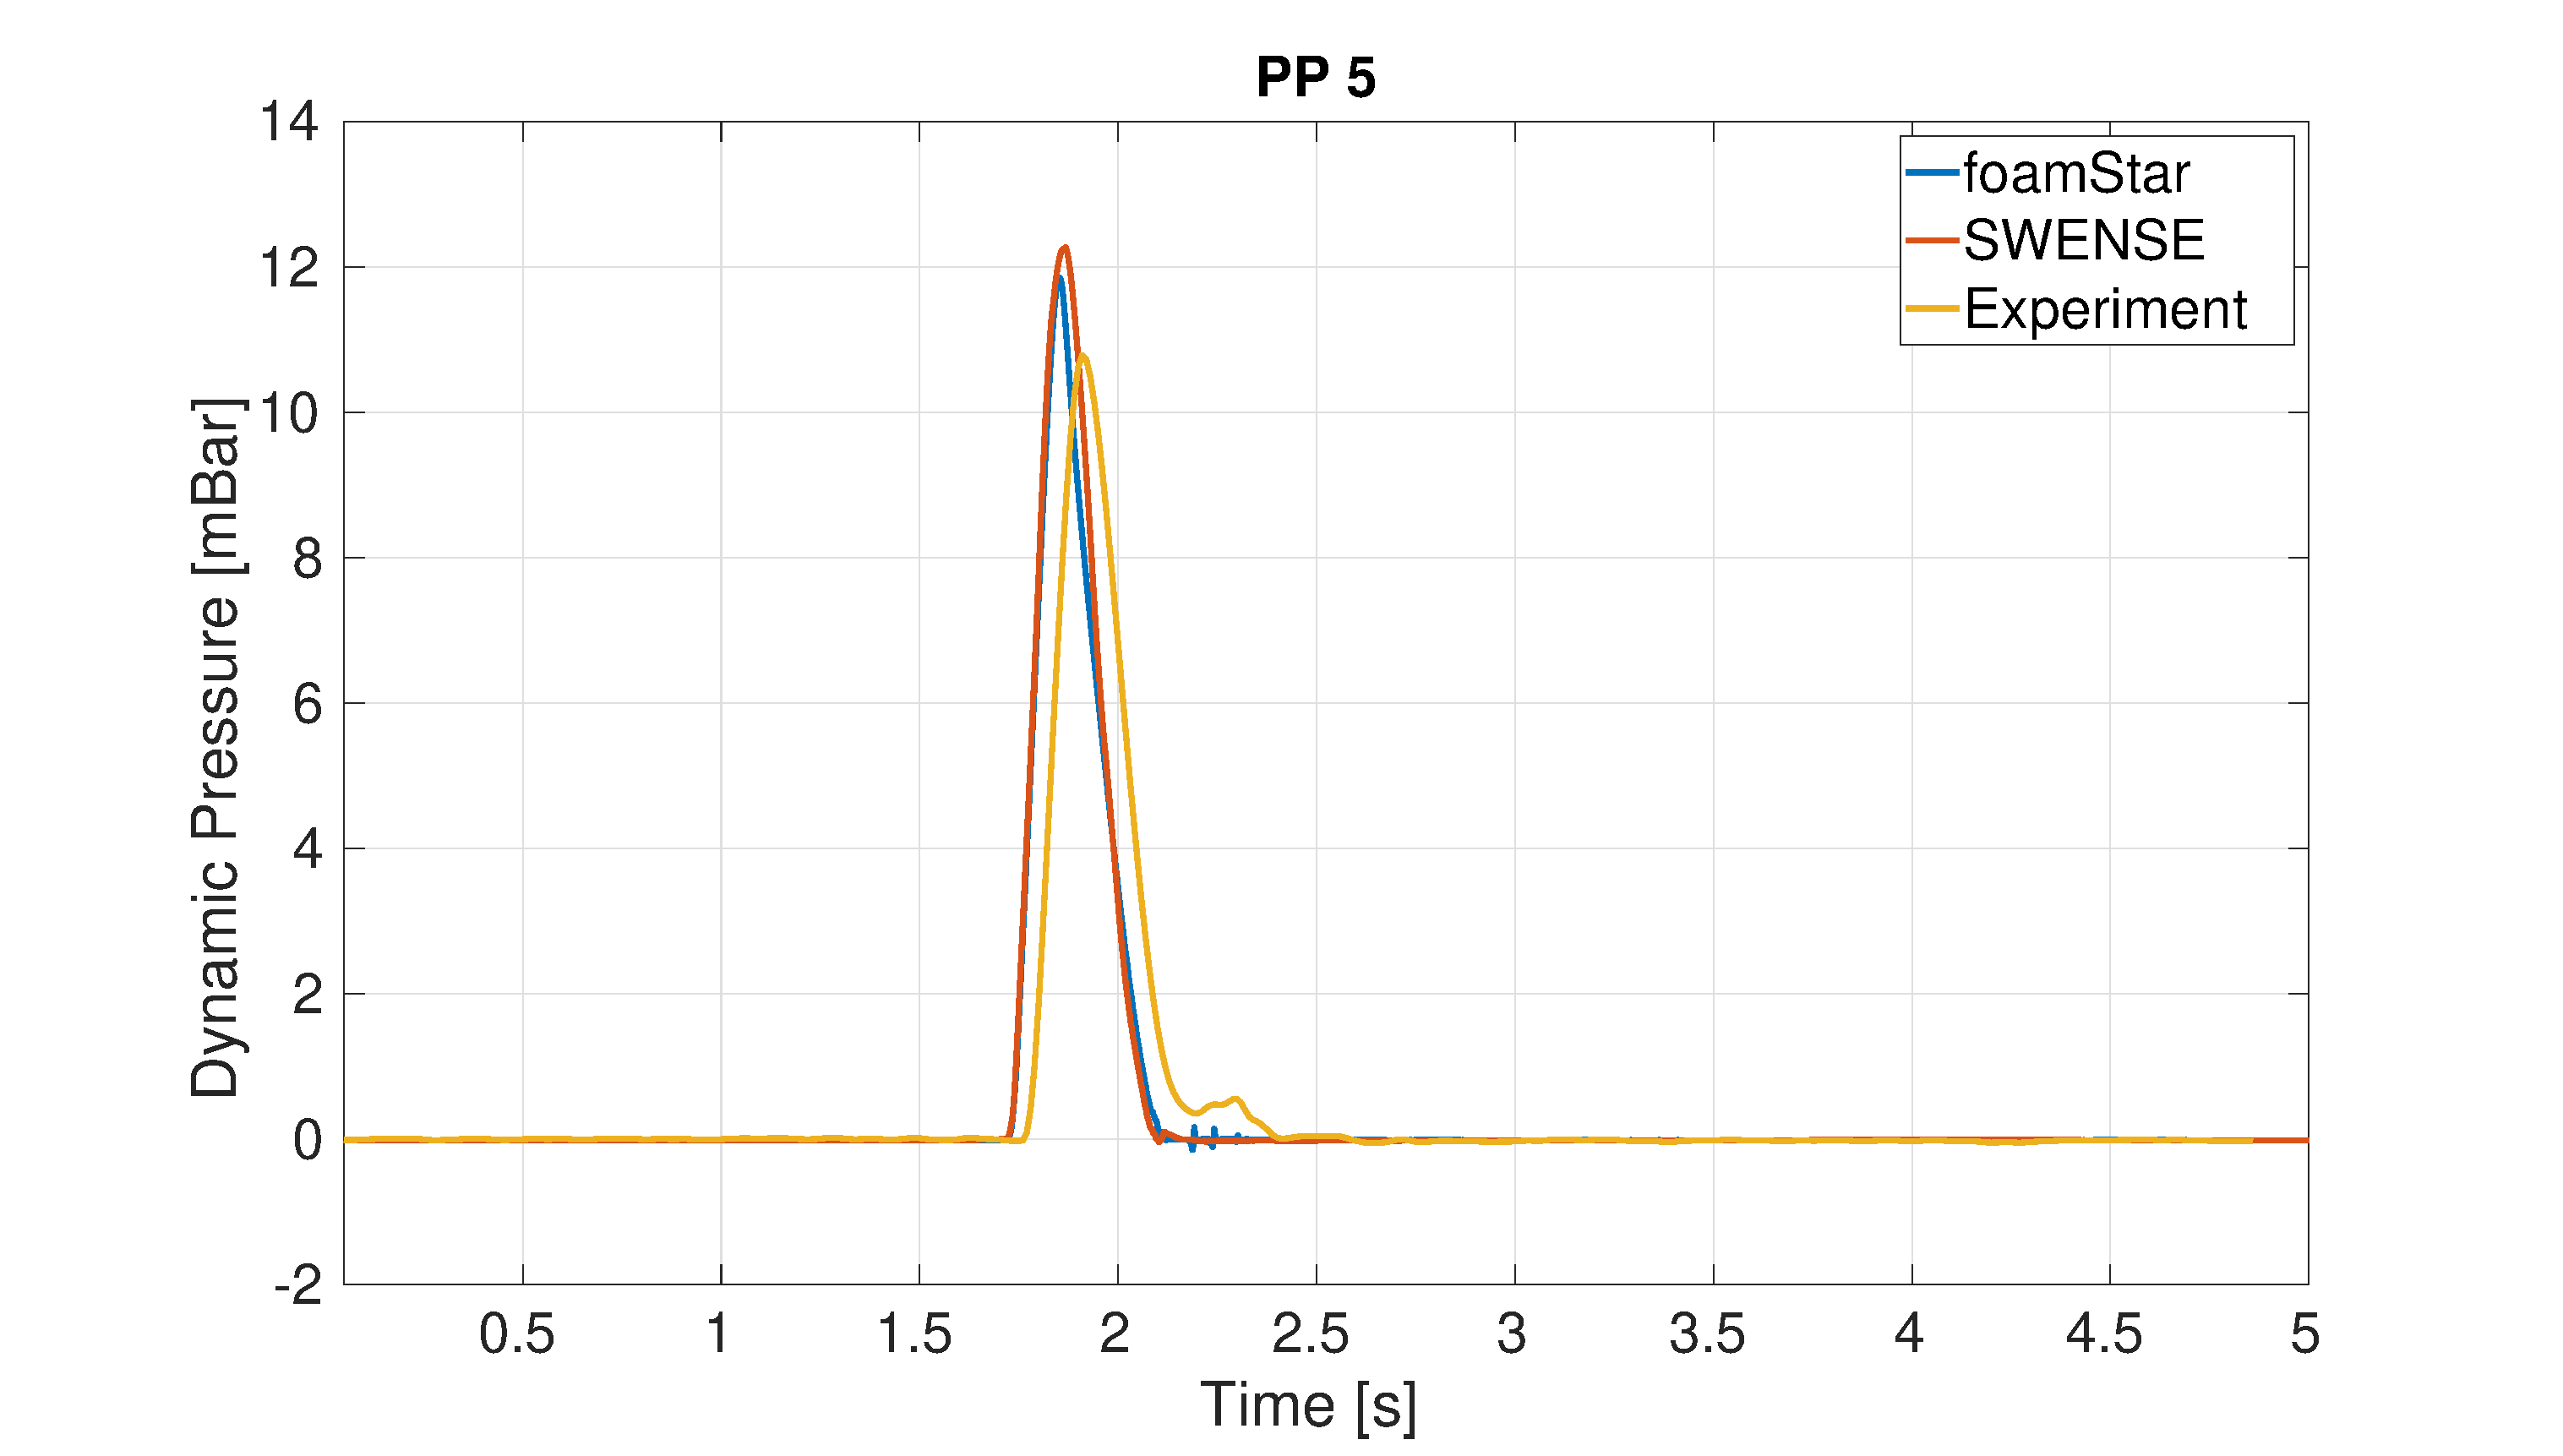
\includegraphics[width=65mm,height=50mm]{PP5.eps}}
	\subfigure[PP6]{\label{Pforce_beam}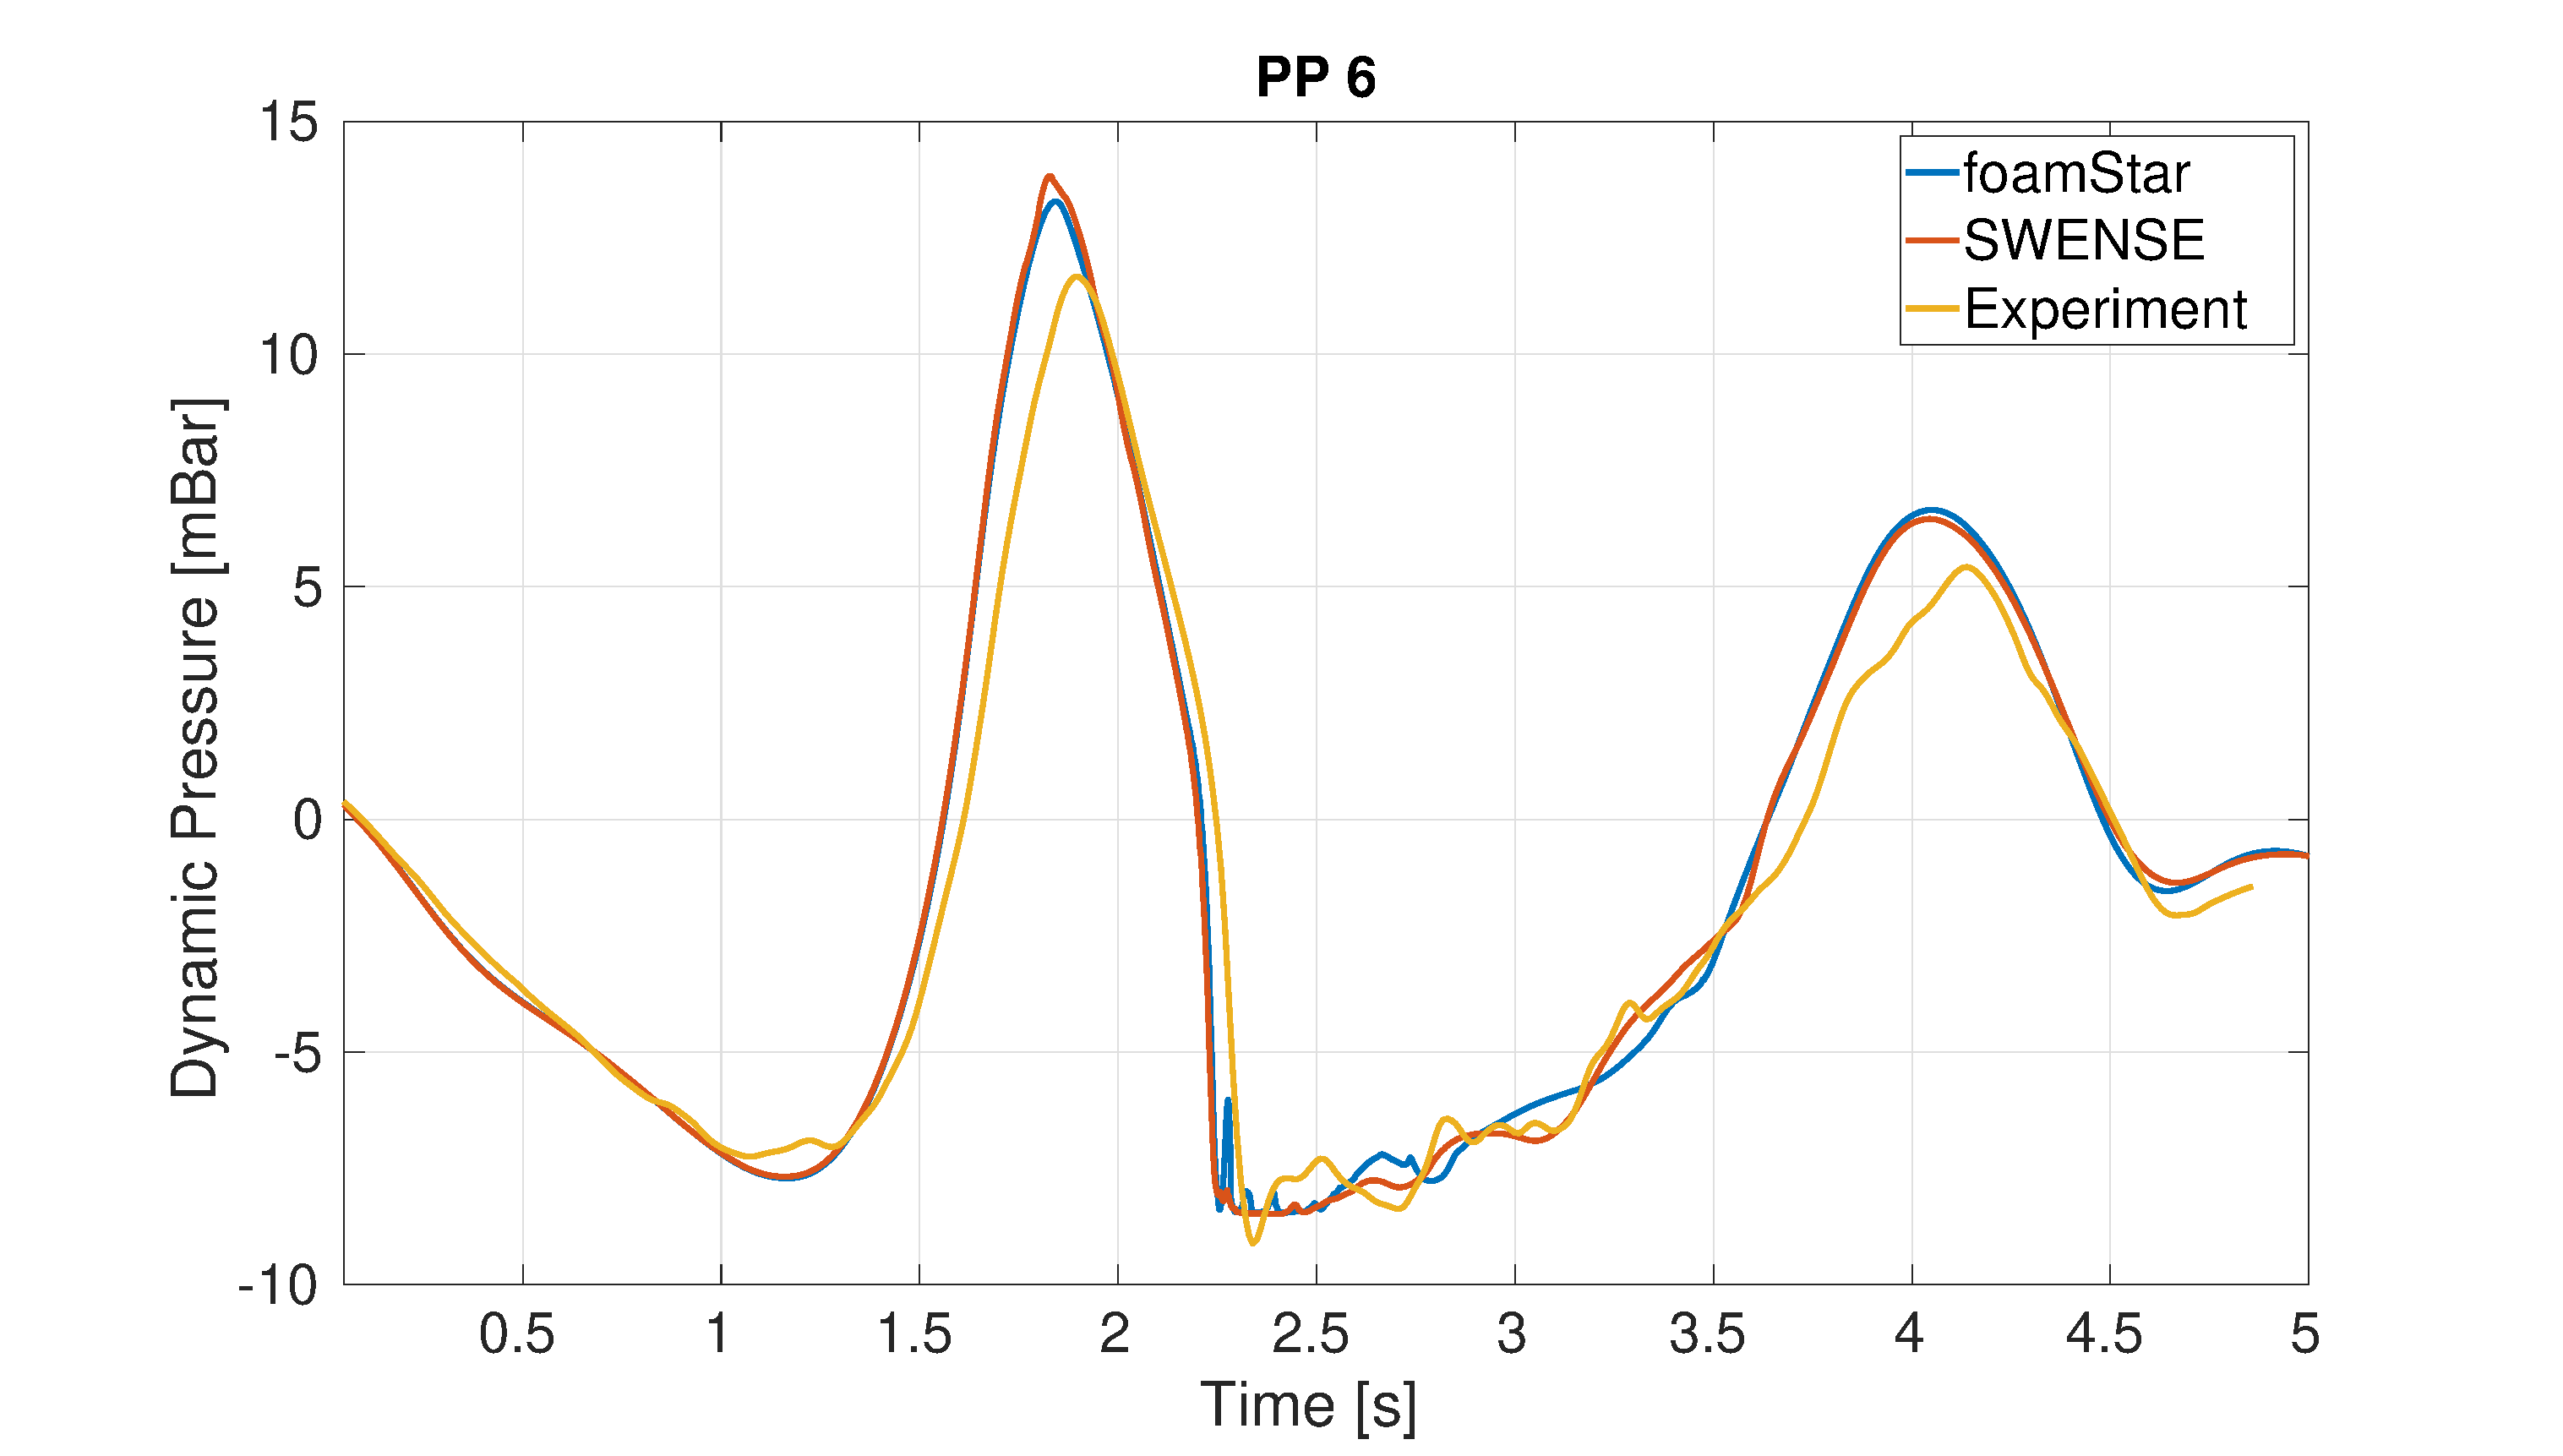
\includegraphics[width=65mm,height=50mm]{PP6.eps}}
	\subfigure[PP7]{\label{Pforce_head}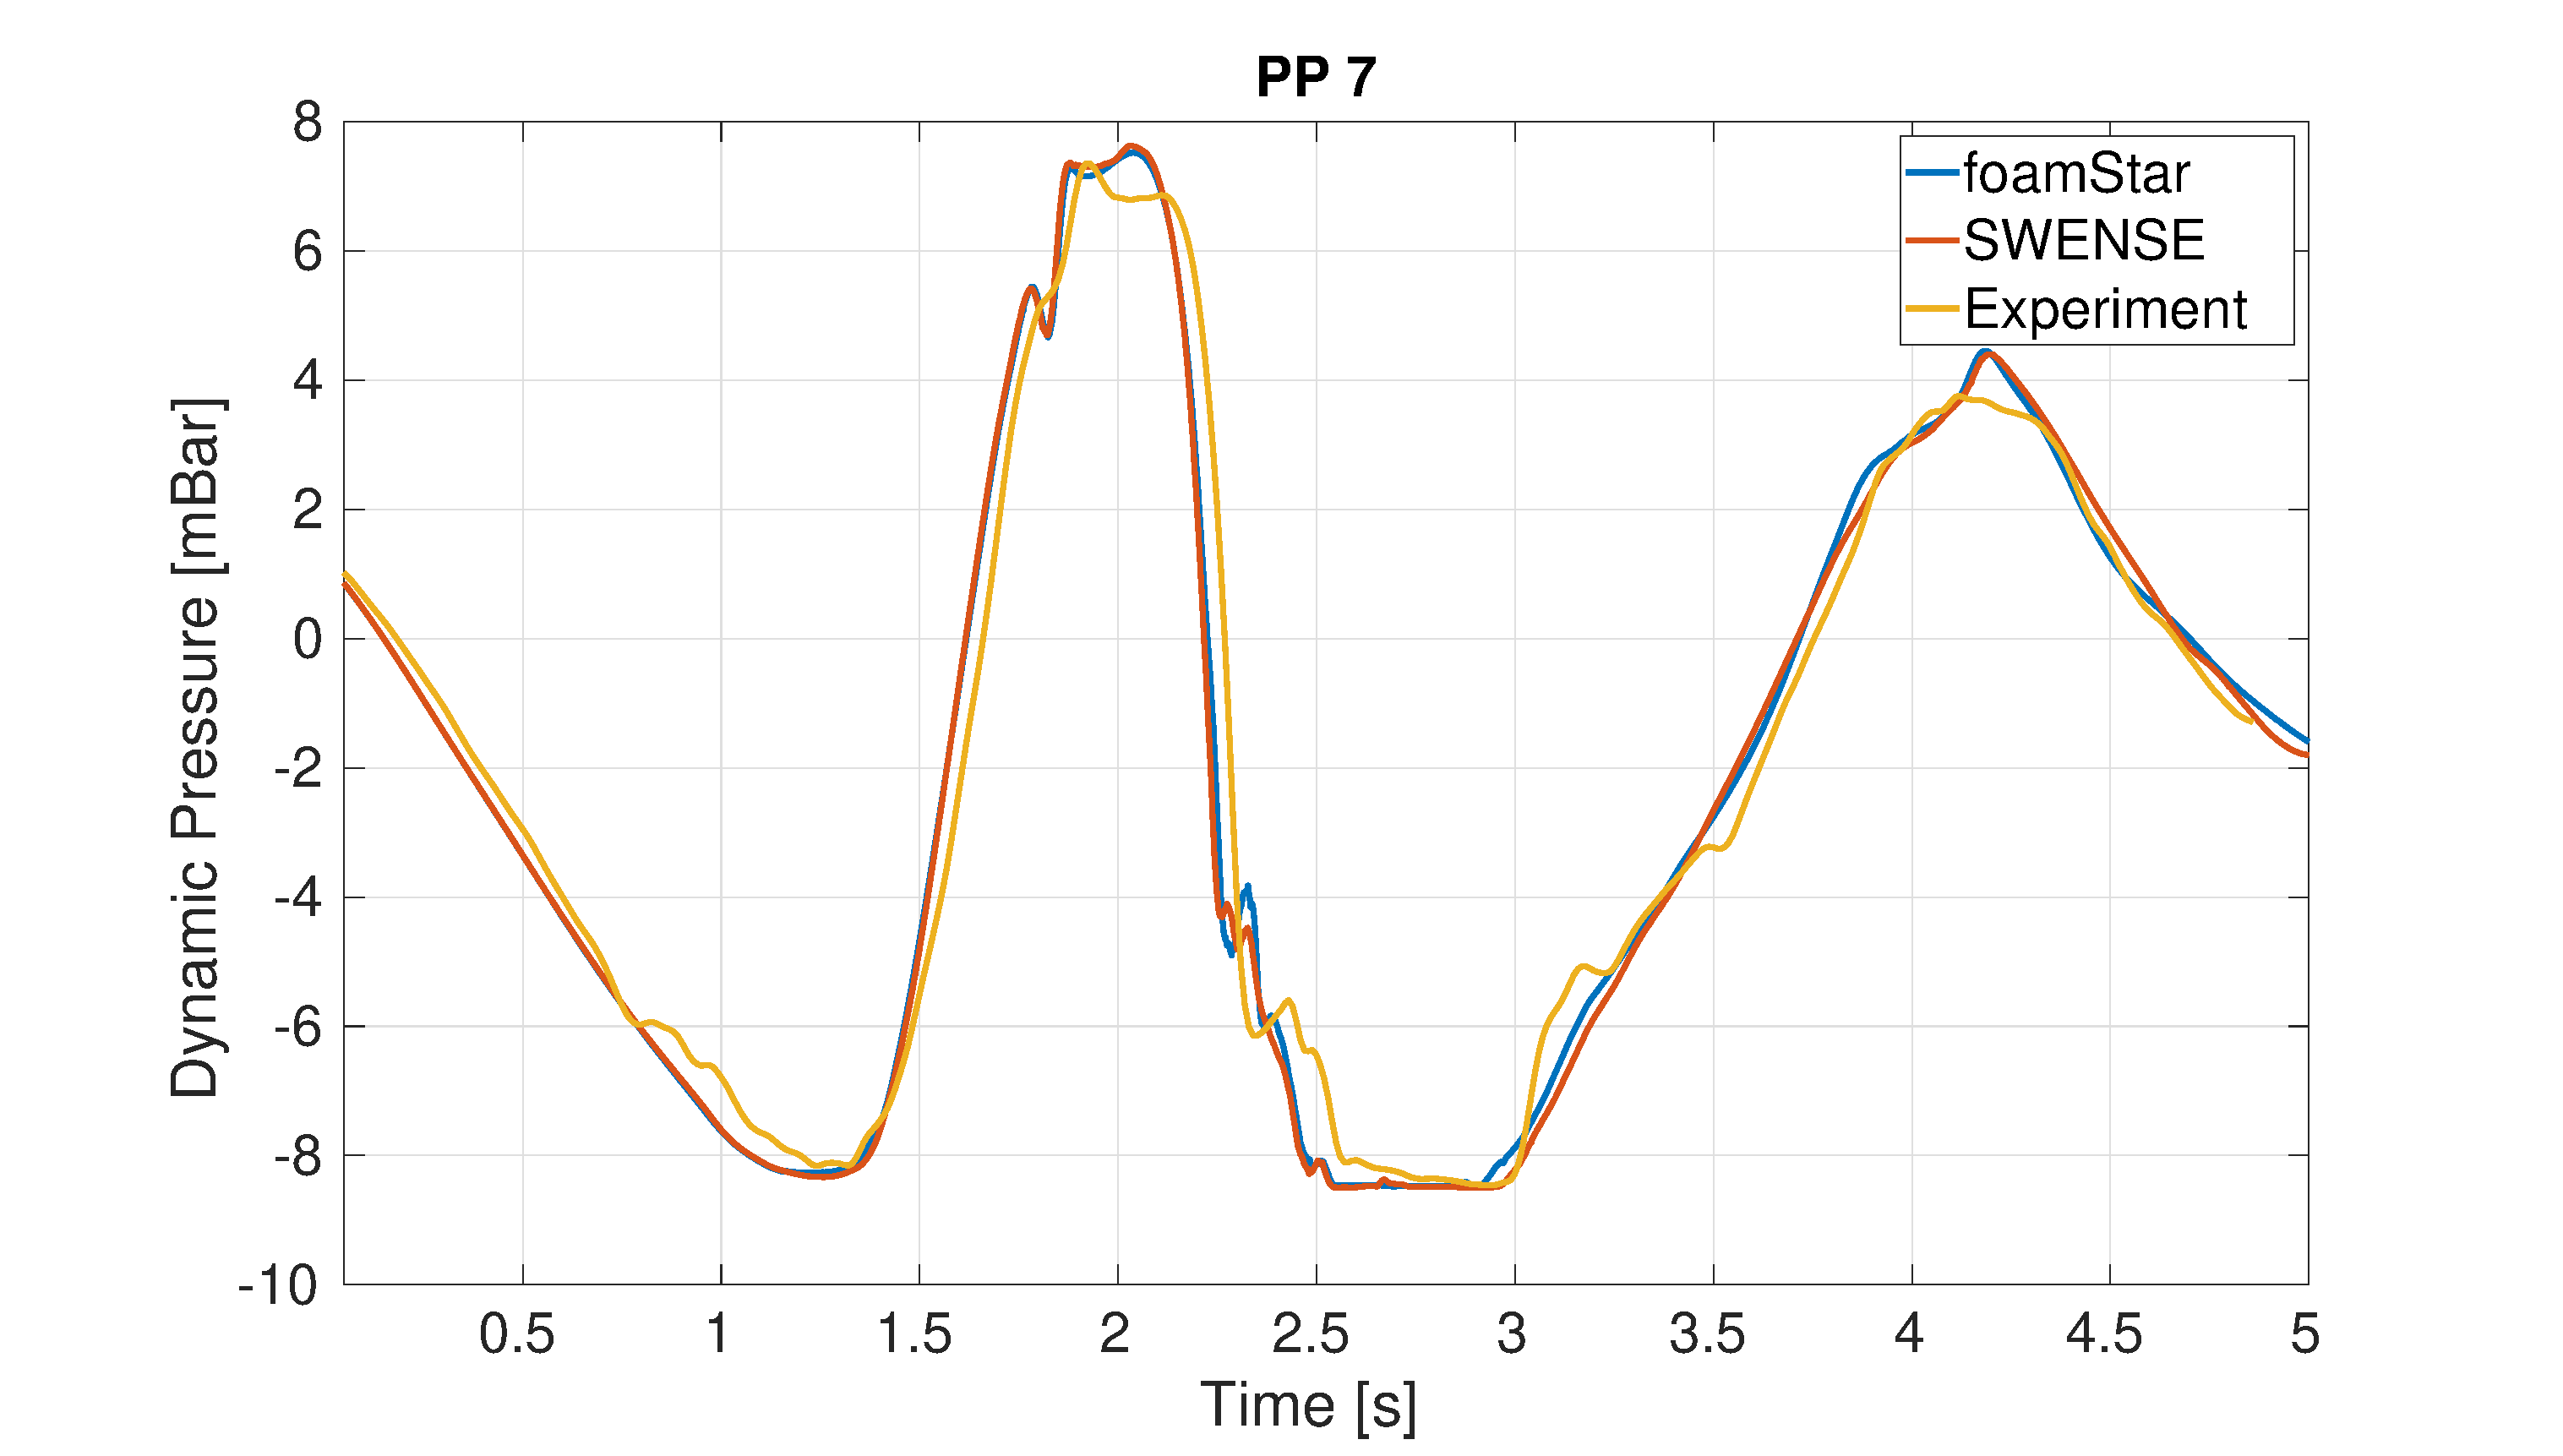
\includegraphics[width=65mm,height=50mm]{PP7.eps}}
	
\caption{Pressure time history comparison for fixed cylinder in non breaking focusing waves between numerical simulation and experiments} \label{fig:NBR_fixed_PP}

\end{figure}


\section{Experimental studies}
	\begin{figure}[H]
	\centering     %%% not \center
	\subfigure
	[Skeleton structure]{\label{WO}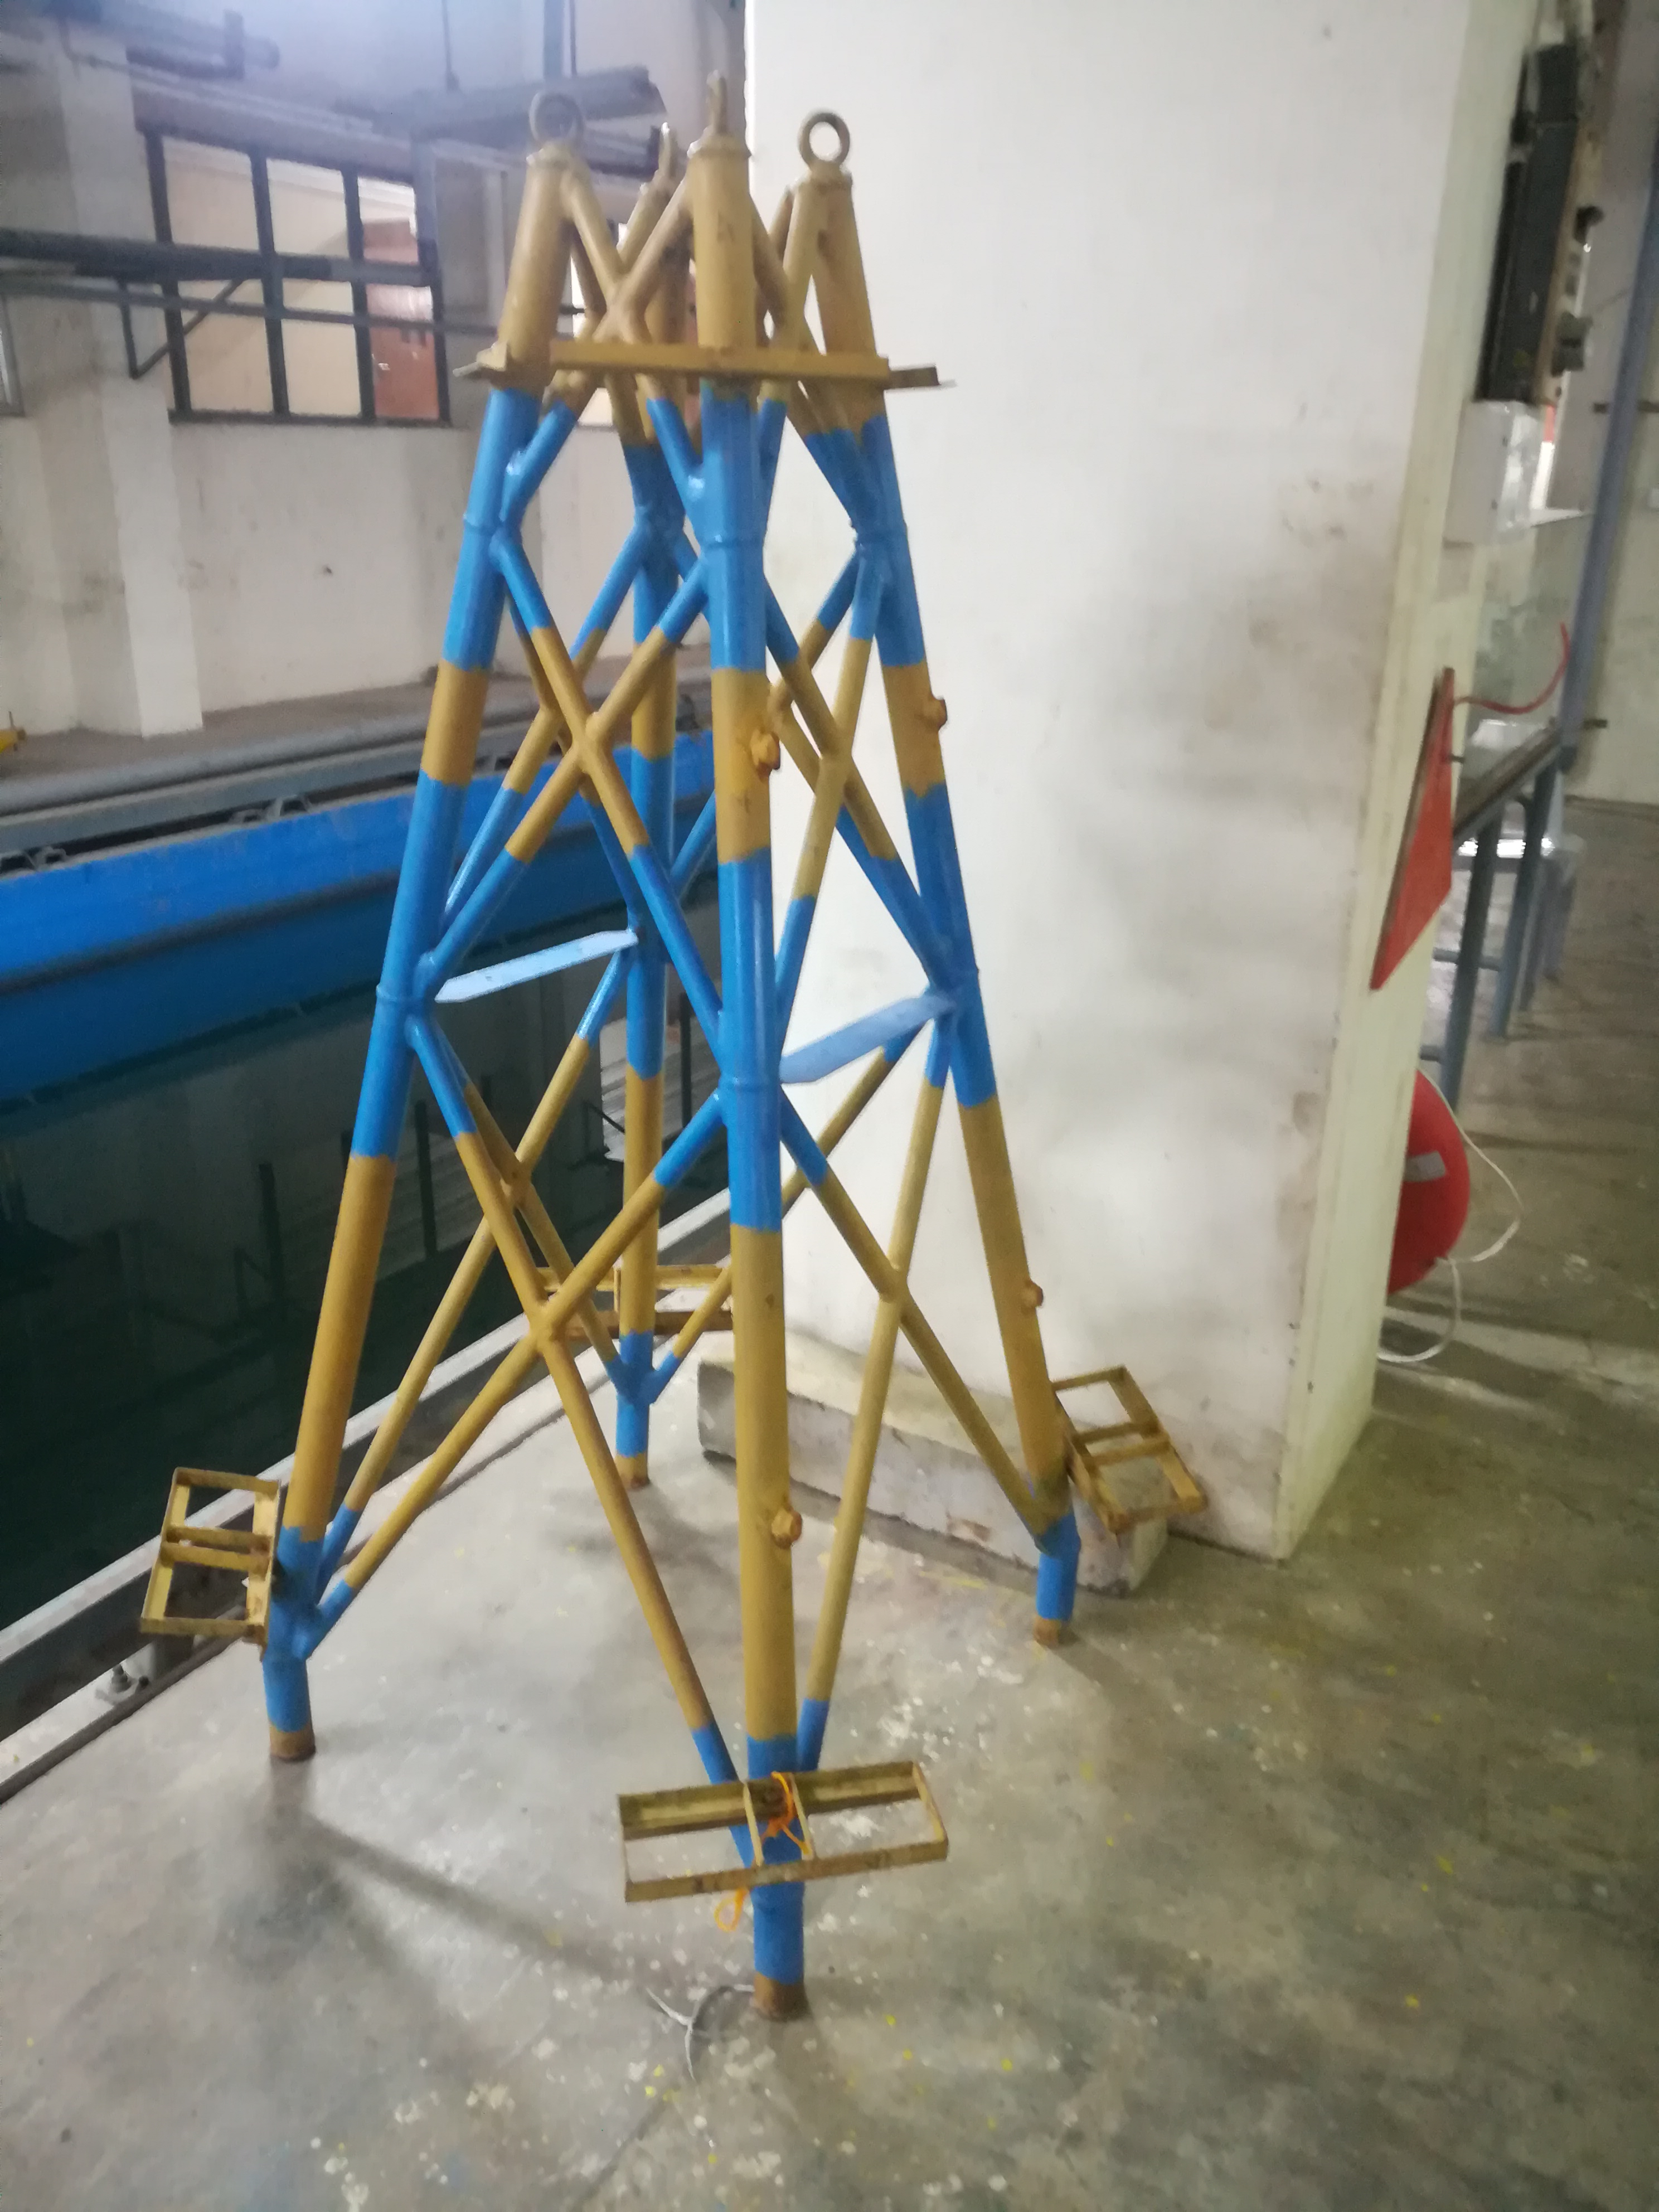
\includegraphics[width=60mm]{WO_buoyancy_tank}}
	\subfigure
	[with buoyancy tank]{\label{WB}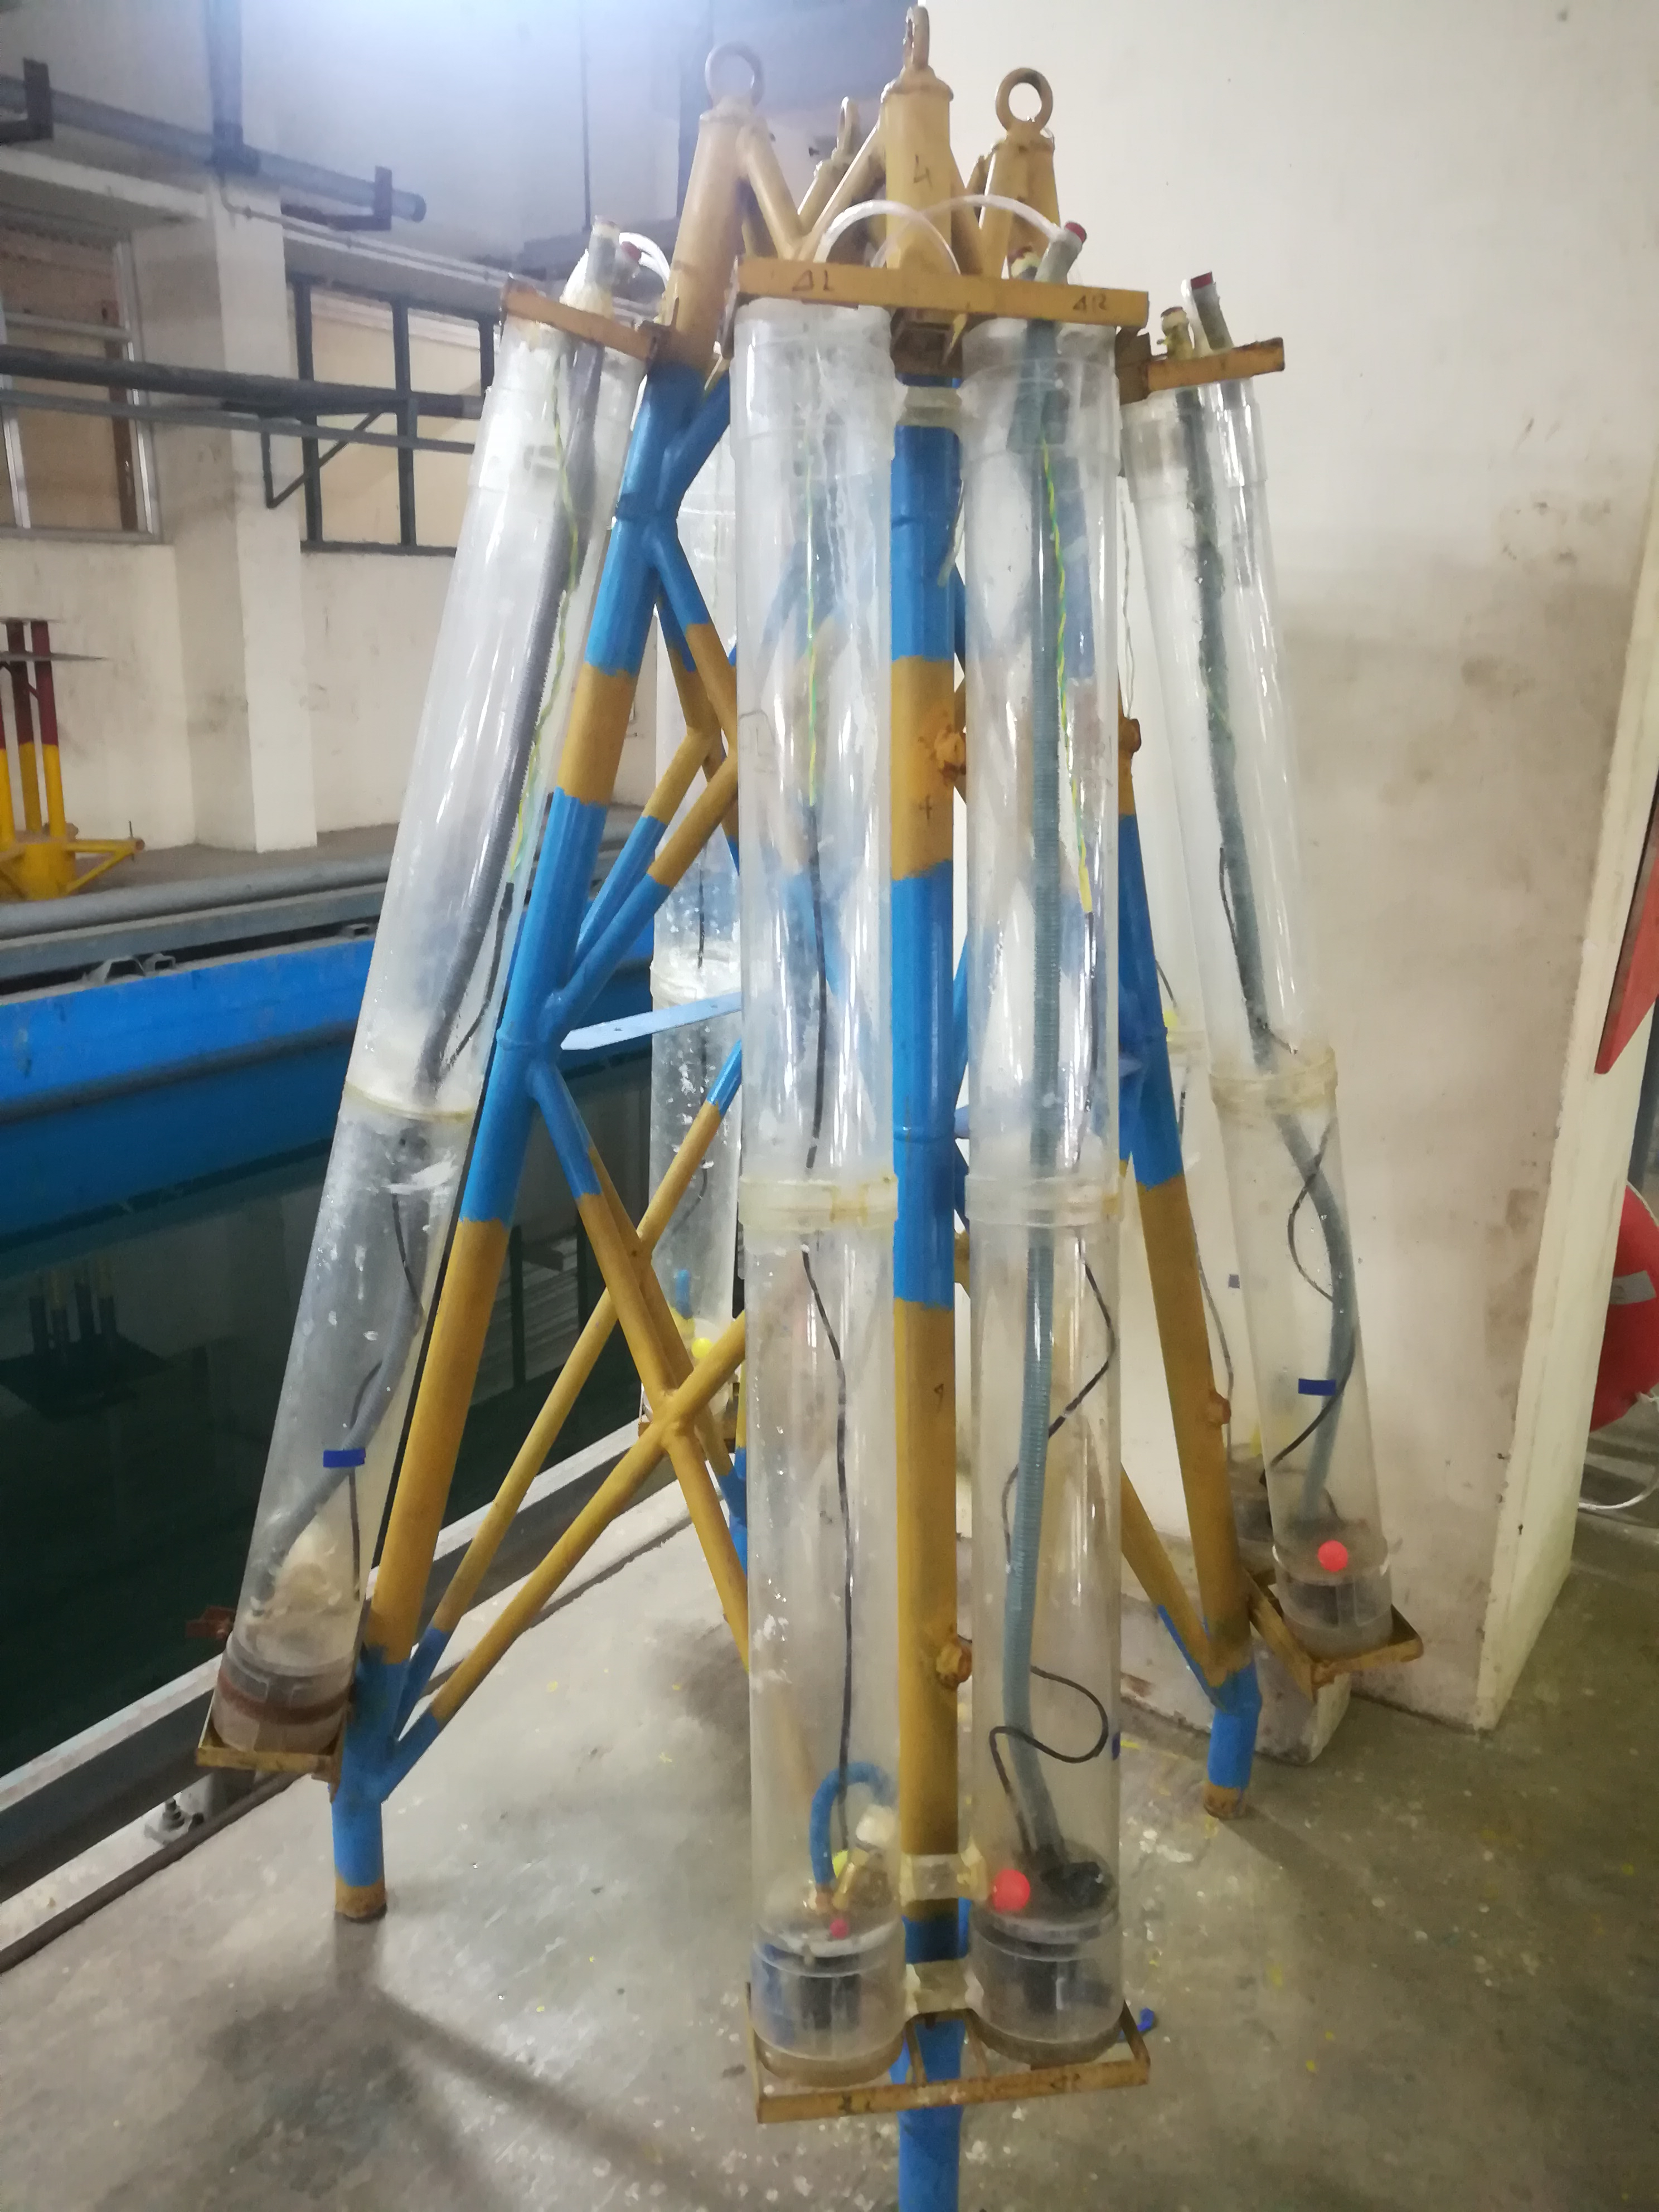
\includegraphics[width=60mm]{W_B_tank}}
	\caption{Experimental jacket model with and without buoyancy tank}
\end{figure}

For the validation of the solver for the complex wave structure interaction, experiment carried out in IITM wave basin will be used. The offshore wind farms substructure is considered to be a concrete jacket, which is different from the conventional steal jacket structure. The physical jacket model used in the experiment with and without buoyancy tank is shown in the Figure \ref{foamStar_validation}. In order to understand its behaviour, two different cases, one as a freely floating and other with crane rope setup is investigated. Further, three different floating positions are carried out, namely, initial stage ($17^o$),mid stage ($45^o$) and vertical stage ($90^o$).  It is observed that the initial stage of upending is more critical compared to other stages of upending. There are considerable results obtained with and without crane rope upending. Experiment details are submitted for journal.  These experimental results will be compared with numerical solvers simulation results in later stages of the research to confirm the solver efficiency. 



\section{Timeline} 

\begin{figure} [H]
    \centering
    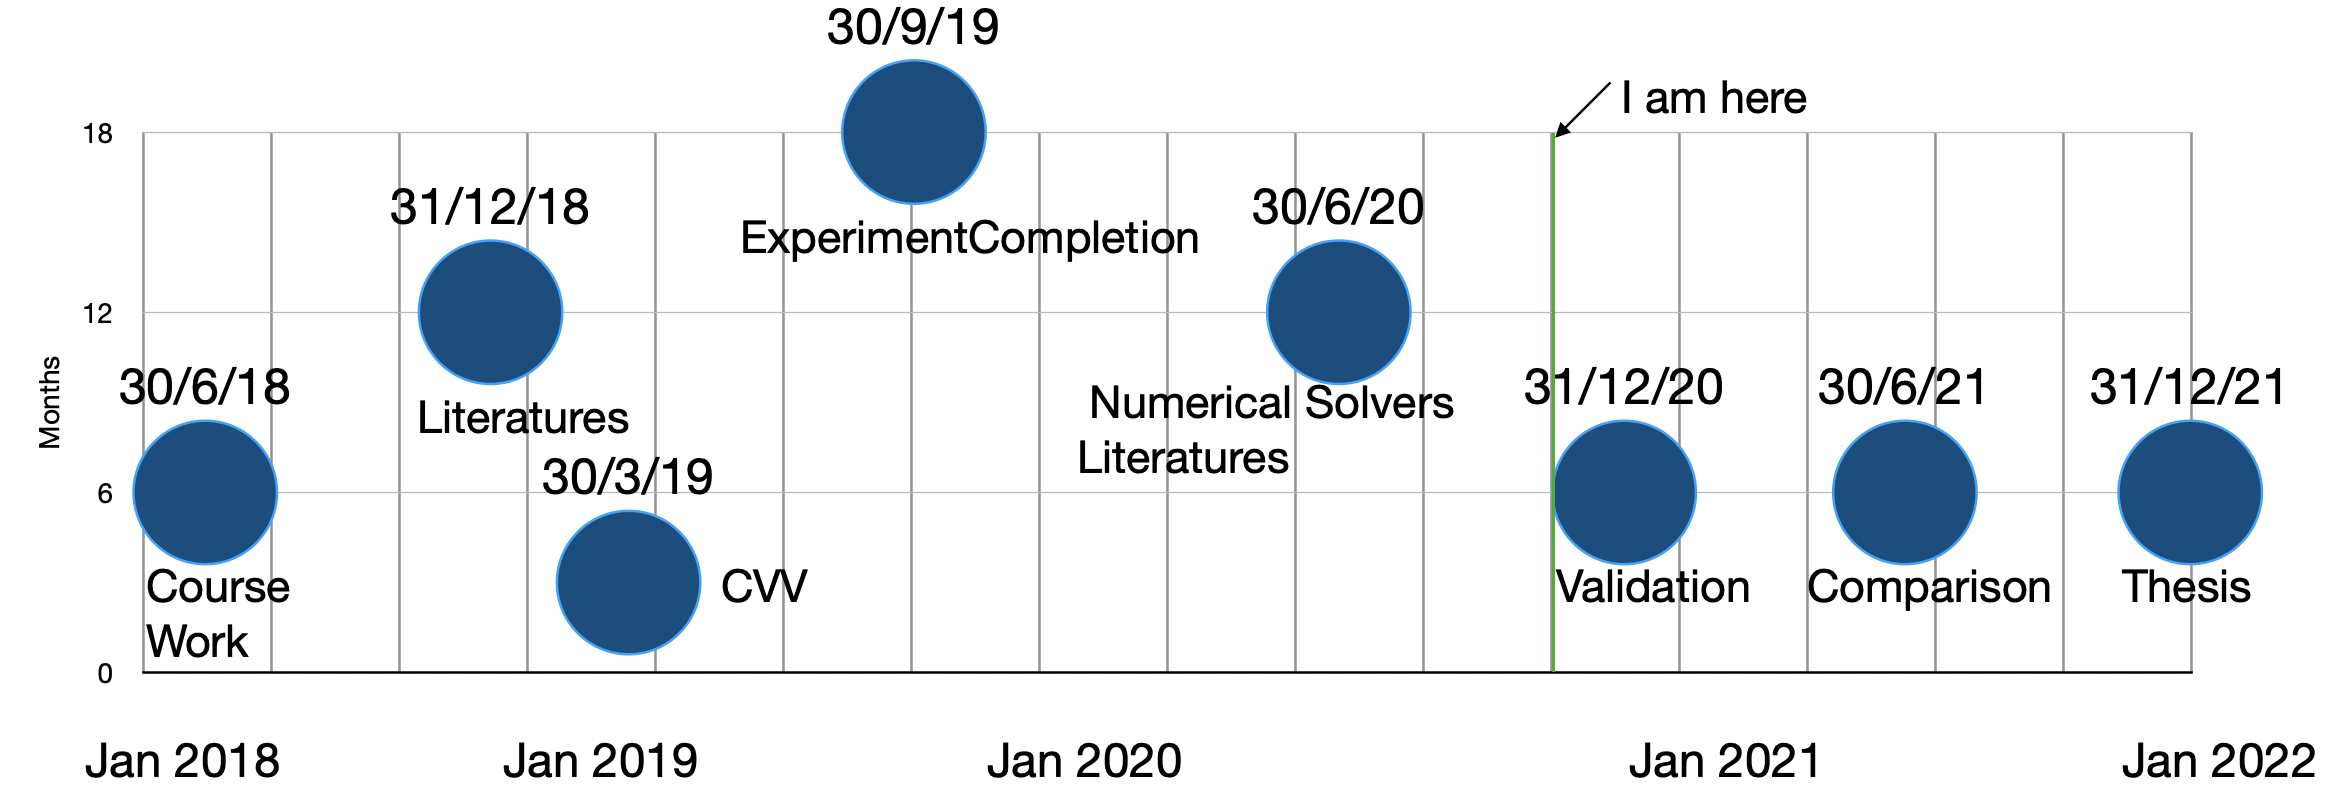
\includegraphics[width=\textwidth]{Timeline1.png}
    \label{Timeline}
\end{figure}






\section{Paper Publication in Journal}
\begin{itemize}
    \item (Submitted,Marine Structures) Experimental investigation offshore crane load during upending a wind turbine jacket sub-structure in regular waves (2019/2020)
    \item (Submitted,IJOPE) Comparative Study on Steep Focused Waves Interactions with moving Cylinder, IJOPE (2020)
    \item (In preparation) Investigation of hybrid coupling capability on complex breaking and nonbreaking focusing waves with fixed and moving cylinder interaction 
\end{itemize}

\addcontentsline{toc}{section}{References}

\bibliographystyle{unsrt}
\bibliography{DomainDecomposition}
}

\end{document}